\documentclass[a4paper]{article}
\title{iCASE PhD report}
\author{David Narganes}
\date{\today}


\usepackage{mathtools}          % mathematics notation
\usepackage{graphicx}           % manipulation of images
\usepackage{booktabs}           % tables
\usepackage{multicol}           % multiple columns
\usepackage{float}              % pictures in place
\usepackage{hyperref}
\usepackage{amssymb}
\usepackage{listings}
\usepackage{array}
\usepackage[a4paper,bindingoffset=0.2in,%
            left=0.8in,
            right=0.8in,
            top=0.8in,
            bottom=0.8in,
            footskip=.25in]{geometry}

\hypersetup{
    colorlinks=true,
    citecolor=red,
    linkcolor=blue,
    urlcolor=blue,
}

\usepackage{color}
\definecolor{codegreen}{rgb}{0,0.9,0}
\definecolor{codegray}{rgb}{0.4,0.4,0.5}
\definecolor{codepurple}{rgb}{0.58,0,0.82}
\definecolor{backcolour}{rgb}{0.95,0.95,0.97}
 
\lstdefinestyle{mystyle}{
    backgroundcolor=\color{backcolour},   
    commentstyle=\color{codegreen},
    keywordstyle=\color{red},
    stringstyle=\color{codepurple},
    basicstyle=\footnotesize,
    breakatwhitespace=false,         
    breaklines=true,                 
    captionpos=b,                    
    keepspaces=true,                 
    showspaces=false,                
    showstringspaces=false,
    showtabs=false,                  
    tabsize=2
}
\lstset{style=mystyle}

% Defining native folder for pics
\graphicspath{ {./pics/} }

% Length of indentation for the document
\setlength{\parindent}{1cm}
\setlength{\parskip}{0em}

% Shade quotes
\usepackage{framed}
\usepackage{color}
\newenvironment{shadequote}%
{\begin{snugshade}\begin{quote}}
{\hfill\end{quote}\end{snugshade}}
\definecolor{shadecolor}{rgb}{0.9,0.9,0.9}

\begin{document}
\maketitle
\tableofcontents
\newpage

% Introduction
\section{Introduction}
\subsection{Motivation}

Traditionally, in drug discovery, target identification to develop novel agents for any given disease is carried out on a case--by–-case basis. In this model, individual scientists act as project champions for targets based on available literature and local expertise. Nevertheless:

\begin{itemize}
    
    \item With increasing publication rates, it is becoming impossible to maintain an overview over an \textbf{increasingly vast scientific} literature. The large quantity not just biomedical research literature but also orthogonal perspectives continually being produced renders it impossible for individual researchers to keep up to date \cite{brown2018}.
    
    \begin{center}
    \emph{``Every two days we create as much information as we did from the dawn of civilization up until 2003, and the pace is increasing''}
    \end{center}
    \rightline{--- Eric Schmidt, former CEO of Google}
    
    \item In recent years a wealth of biological data from multiple domains has become available in \textbf{public data repositories} \cite{brown2018}. A firm integration of this extensive and extremely valuable corpus of scientific literature is necessary for a rapid generation of new, high-quality hypothesis for drug discovery without the need of human intervention \cite{ferrero2017, brown2018}.
    
    \item Drug discovery is \textbf{extremely costly and failure-prone} \cite{ferrero2017}. As the cost of successful drug development continues to increase, the productivity of the industry as a whole in launching new drugs remains flat \cite{brown2018}.
    
\end{itemize}

Hence, the putative target prioritisation in drug discovery:
\begin{itemize}
    \item Is of paramount importance to maximise the chances of success in clinic \cite{ferrero2017}.
    
    \item Ensures a sustainable business in the long term \cite{ferrero2017}.
\end{itemize}


\subsection{Proposed approach}
Based on the \href{https://goo.gl/QrfdfY}{initial proposal}, this PhD iCASE will focus on:
\begin{itemize}
    \item The development of an innovative integrated resource 
    \item which uses machine learning algorithms
    \item to exploit a newly generated semantic repository
    \item to facilitate a systematic genome scale ranking of potential targets in the areas of both type 2 diabetes and metabolic syndrome: a \textbf{putative therapeutic target priorisation} (PTTP)
\end{itemize}


The project will also explore different ranking systems to prioritize putative targets, for instance:


\begin{itemize}
    \item \textbf{Weighted averages} based on data types results.
    \item \textbf{Network topology} based scores.
    \item \textbf{Machine learning} approaches based on fingerprints derived from datatypes.
    \item \textbf{Enrichment} of the semantic repository with text mining approaches, linking to electronic medical records (EMR) or genomic resources available at the School of Medicine.
\end{itemize}

The different approaches for the target ranking can be evaluated by their ability to identify or prioritise a gold standard data set of targets provided by Exscientia.
\newpage

% Related work
\section{Related work}
Several resources have been developed to provide comprehensive information on GDAs by integrating multiple data sources:
\begin{itemize}
    \item DrugBank \cite{drugbank2008}
    \item Therapeutic Target Database \cite{ttd2018}
    \item STITCH \cite{stitch42014}
    \item PharmaGKB \cite{pharmaGSK2012}
    \item SuperTarget \cite{superTarget2012}
\end{itemize}

The emphasis of these databases is on the known and predicted interactions between the clinical trial drugs and their targets, how drug effects on targets are propagated through their corresponding pathways, their relationships to diseases, adverse events of drugs and pharmacogenomics \cite{brown2018}. They do not provide a \emph{Putative Therapeutic Target Priorisation} (\textbf{PTTP}). Nevertheless, there has been some attempts to develop a more systematic approach (see Table \ref{tab:related_work}).

\begin{table}[H]
\centering
    \begin{tabular}{c|c|c}
      GDA Initiative & Section & Citation \\
      \hline
      
      \href{https://goo.gl/ewnpWZ}{DisGeNET} & \ref{subsec:DisGeNET} & \cite{DisGeNET2015} \\
      
      \href{https://goo.gl/KGQsd9}{DISEASES} & \ref{subsec:DISEASES} & \cite{DISEASES2015} \\
      
      \href{https://goo.gl/eQ667p}{Open Targets} & \ref{subsec:ot} & \cite{koscielny2016} \\
      
      \href{https://goo.gl/dPWHNY}{PHAROS} &  \ref{subsec:pharos} & \cite{pharos2016} \\
      
      \href{https://goo.gl/edKMH7}{Open PHACTS} & & \\
      
      \end{tabular}
\caption{PTTP initiatives, section in the report, and publication \label{tab:related_work}}
\end{table}

% DisGeNET
\newpage
\subsection{DisGeNET} \label{subsec:DisGeNET}
\href{https://goo.gl/ewnpWZ}{DisGeNET} is a discovery platform designed to address questions concerning the genetic underpinning of human diseases by analysing GDAs \cite{DisGeNET2015}. It is maintained by the Integrative Biomedical Informatics (IBI) Group at the Universitat Pompeu Fabra in Barcelona, Spain. DisGeNET made a clear distinction between Gene--Disease Associations (GDAs) and Variant--Disease Associations (VDAs) even though VDA is a GDA subclass in their ontology (see Figure \ref{fig:disgenet_ontology}). Is not VDA a subclass of GDA like they explain in the ontology in their ontology in Figure \ref{fig:disgenet_ontology} ?

\subsubsection{Data sources}
DisGeNET is organised according to the type and level of curation (see Table \ref{tab:disgenet_data} and \href{https://goo.gl/ntXTjX}{DisGeNET statistics}. For simplicity and given that they consider GDA as a VDA parent in the DisGeNET ontology (see Figure \ref{fig:disgenet_ontology}), I will just consider VDAs as a subtype of GDAs that includes the \texttt{Genomic Alterations} class and their children: any SNP, deletion, insertion, indel, somatic SNV, substitution, sequence alteration, or tandem repeat.

\begin{table}[H]
    \centering
    \resizebox{\textwidth}{!}{
    \begin{tabular}{c|c|c|c|c|c}
    Source & Type & Genes & Diseases & GDAs & Description \\
    \hline
    
    \href{https://goo.gl/XtufGc}{UniProt} &
    C & 19027 & 6303 & 20722 &
    Curated protein functional information \cite{uniprot2017} \\
    
    \href{https://goo.gl/aTyMBE}{CTDh} &
    C & 7787 & 4929 & 25975 &
    Environmental chemicals, genes and diseases \cite{ctd2017} \\
    
    \href{https://goo.gl/89TfbR}{ClinVar} &
    C & 45546 & 5639 & 54888 &
    Genetic human variants and diseases \cite{clinvar2016} \\
    
    \href{https://goo.gl/KxxD8Y}{GWASC} &
    C & 15790 & 610 & 20719 &
    GWAS catalog \cite{gwasCatalog2017} \\
    
    \href{https://goo.gl/hUkKLf}{Orphanet} &
    C & 2661 & 6702 & 97547 &
    Rare disorders, genes, and orphan drugs \cite{orphanet2012} \\

    \href{https://goo.gl/mgFWK4}{PsyGeNET} &
    C & 1546 & 112 & 3757 &
    Psychiatric GDAs \cite{PsyGeNET2015} \\

    \href{https://goo.gl/gYHKF3}{HPO} &
    C & 2661 & 6702 & 97547 &
    Phenotypic vocabulary for human diseases \cite{humanPhenotypeOntology2014} \\
    
    \href{https://goo.gl/aTyMBE}{CTDr} &
    M & 22 & 13 & 31 &
    CTD for \textit{Rattus Norvergicus} \cite{ctd2017} \\
    
    \href{https://goo.gl/aTyMBE}{CTDm} &
    M & 22 & 13 & 31 &
    CTD for \textit{Mus Musculus} \cite{ctd2017} \\
    
    \href{https://goo.gl/zc52JW}{RGD} &
    M & 1076 & 629 & 4291 &
    Genomic and disease data of \textit{R Norvegicus} \cite{rgd2015} \\
    
    \href{https://goo.gl/iTNmRx}{MGD} &
    M & 1464 & 1323 & 1994 &
    Genomic and disease data of \textit{M Musculus} \cite{mgd2015} \\
    
    \href{https://goo.gl/y3keCN}{GAD} &
    L & 13318 & 3099 & 63063 &
    GWAS repository \cite{gad2004}. Retired on 09/01/2014 \\
    
    \href{https://goo.gl/szDDw6}{LHGDN} &
    L & 5941 & 1799 & 31468 &
    Semantic ML extraction of GDAs \cite{bundschus2008} \\
    
    \href{https://goo.gl/4Yau27}{BeFree}* &
    L & 35392 & 16274 & 453574 &
    Biomed Name-Entity Recogniser of GDAs \cite{bravo2015} \\
    
    Total &  & 100076 & 29539 & 696707 \\
    
    \end{tabular}}
    \caption{Original data sources used by DisGeNET v5.0 \cite{DisGeNET2015}, type (\textbf{C} for curated data sources, \textbf{M} for Animal model data sources, and \textbf{L} for literature evidence sources), number of genes or gene variants, number of diseases or phenotypes, number of Gene--Disease Associations (GDAs or VDAs) and brief description. Information obtained from
    \href{https://goo.gl/ntXTjX}{DisGeNET statistics} \label{tab:disgenet_data}}
\end{table}

*The document used to extract GDAs was defined by the following PubMed query:

\begin{center}
\emph{
\small{
("Psychiatry and Psychology Category"[Mesh] AND "genetics"[Subheading]) OR ("Diseases Category"[Mesh] AND "genetics"[Subheading]) AND (hasabstract[text] AND ("1980"[PDAT] : "2017"[PDAT]) AND "humans"[MeSH Terms] AND English[lang])
}
}
\end{center}


\subsubsection{Scores}
DisGeNet developed two different confidence scores\footnote{\url{https://goo.gl/aSJVAd}}: one for GDAs and another for VDAs that reflected the evidence across all data sources \cite{DisGeNET2015}. I simplified the formulas they used, also because they are wrong: VDA has just two literature sources (GAD and BeFree), it cannot be a sum of three sources. Both scores ranges form 0 to 1 and the explanation of the variables is in Table \ref{tab:equationDisgenet}:

$$ score_{gda} = C + M + \sum_{l=1}^3 L_l $$
$$ score_{vda} = C + \sum_{b=1}^2 B_b $$

Note that the values for $C$ are different between GDA and VDA, I have not described the different values for VDA. Where:

\[
C =
\left\{
 \begin{array}{l}
  0.6 \quad if \quad c > 2 \\
  0.4 \quad if \quad c = 2 \\
  0.2 \quad if \quad c = 1 \\
  0.0 \quad otherwise
 \end{array}
\right.
\]

\[
M =
\left\{
 \begin{array}{l}
  0.16 \quad if \quad m = 2 \\
  0.08 \quad if \quad m = 1 \\
  0.00 \quad otherwise
 \end{array}
\right.
\]

\[
L =
\left\{
 \begin{array}{l}
  0.08 \quad if \quad 100 \cdot R_l \geq 0.08 \\
  R_l \quad\quad if \quad 100 \cdot R_l < 0.08
 \end{array}
\right.
\]

\[
B =
\left\{
 \begin{array}{l}
  0.15 \quad if \quad 100 \cdot R_b \geq 0.15 \\
  R_b \quad\quad if \quad 100 \cdot R_b < 0.15
 \end{array}
\right.
\]

\begin{table}[H]
    \centering
    \resizebox{\textwidth}{!}{
    \begin{tabular}{c|c}
    Variable & Meaning \\
    \hline
    
    $c$ & Number of curated, GDA--suporting sources: Uniprot, CTD, Orphanet, PsyGeNet, HPO \\
    $m$ & Number of animal models supporting GDA: \textit{M musculus} and \textit{R Norvegicus} \\
    $R_l$ & Ratio between GDA supporting papers and total papers in the data source $l$ \\
    $l$ & Index for GDA literature sources: GAD, LHGDN, BeFree \\
    $R_b$ & Ratio between VDA supporting papers and total papers in the data source $b$ \\
    $b$ & Index for VDA literature sources: GAD, BeFree
    \end{tabular}}
    \caption{Meaning of the variables for the GDA score in DisGeNET \label{tab:equationDisgenet}}
\end{table}

Why do they define this arbitrary weights for the data types? Why do not they assess the variability of each data type to define clusters in an unsupervised method? Why they do not use \href{https://goo.gl/k6vEBj}{information or entropy gain methods} like Open Targets \cite{ferrero2017} to assign a weight of each data type?

\subsubsection{Disease Specificity Index (DSI)}
\label{subsubsec:dsi}
Genes can potentially be associated to multiple diseases (e.g. TNF) while genes are associated to a reduced number of diseases or even to a single disease \cite{DisGeNET2015}. The disease specificity index (DCI) is defined as:

$$ DSI = \frac{log_2(n) - log_2(N)}{log_2(1) - log_2(N)} $$

Why did they use this complicated formula? Why not the ratio of related diseases and total diseases? They could have taken the inverse to achieve the same ranking in a faster way. Demonstrated in a \href{https://goo.gl/zsegji}{Jupyter notebook} that their formula takes a 2-fold more time than mine.

$$ DSI_{david} = N / n $$

where $N$ is the total number of diseases in DisGeNET (20,370) and $n$ is the number of diseases associated to a given gene \cite{DisGeNET2015}. Example: TNF is associated to more than 1500 diseases, therefore $ DSI_{TNF} = 0.247 $

\subsubsection{Disease Pleiotropy Index (DPI)}
\begin{shadequote}
\textbf{Pleiotropy} (from Greek $\pi\delta\epsilon\iota\omega\nu$ or \emph{pleion}, "more", and $\theta\rho o\pi o\zeta$ or tropos, "way") occurs when one gene influences two or more seemingly unrelated phenotypic traits.
\end{shadequote}
The rationale is similar to the DSI in Section \ref{subsubsec:dsi}, but they considered the number of different MeSH disease classes of the diseases associated to a given gene and the total number of MeSH diseases classes in DisGeNET \cite{DisGeNET2015}. The disease pleiotropy index (DPI) is defined as:

$$ DPI = n_p / N_p $$

where $N_p$ is the total number of MeSH disease classes in DisGeNET (28) and $n_p$ is the number of different MeSH disease classes associated to a given gene \cite{DisGeNET2015}. Example: gene KCNT is associated to 5 different MeSH classes, even though it is also associated to 12 diseases, 2 disease groups, and 2 phenotypes. Therefore $DPI_{KCNT1} = 5/28 = 0.179$.

\subsubsection{Evidence Index}
The evidence index (EI) indicates the existence of contradictory results in publication from BeFree and PsyGeNET supporting GDAs. It is defined as:

$$EI = \frac{n_p}{N}$$

where $n_p$ is the number of publications that support a GDA whereas $N$ is the total number of publication with any evidence (positive or negative) regarding the same GDA.

\subsubsection{Disease Mapping}
DisGeNET used the Unified Medical Language System (UMLS) vocabulary. The repositories of GDAs use different disease vocabularies:
\begin{itemize}
    \item UniProt, CTD, and MGD use OMIM terms
    \item CTD, LHGDN, and RGD use MeSH
    \item CLINVAR and PsyGeNET use UMLS Concept Unique Identifiers (CUIs)
    \item GWAS Catalog uses EFO
    \item Orphanet identifiers were mapped using Orphanet cross--references
    \item GAD disease names were normalised with the UMLS Metathesaurus
\end{itemize}

\subsubsection{Gene Mapping}
For human genes, HGNC symbols (used for some entries in GAD), and Uniprot accession numbers (used by Uniprot) were converted to NCBI Entrez gene identifiers using an in--house dictionary that cross--references HGNC, Uniprot and NCBI-Gene information.

For mouse and rat genes, they used files \texttt{HOM\_MouseHumanSequence.rtp} and \texttt{RGD\_ORTHOLOGS.rtp} to map rat and mouse Entrez gene identifiers to human Entrez identifiers, respectively. These files are available somewhere else\footnote{\url{https://goo.gl/BJuBzY}}. Rat and mouse genes without human ortholog were discarded.

\subsubsection{Association Type Ontology}
For a seamless integration of GDAs data, they developed the DisGeNET association type ontology. All association types as found in the original source databases were formally structured from a parent \texttt{Gene Disease Association} class if there was a relationship between the gene/protein and the disease, and represented as ontological classes (see Figure \ref{fig:disgenet_ontology}).

\begin{figure}[H]
    \resizebox{\textwidth}{!}{
    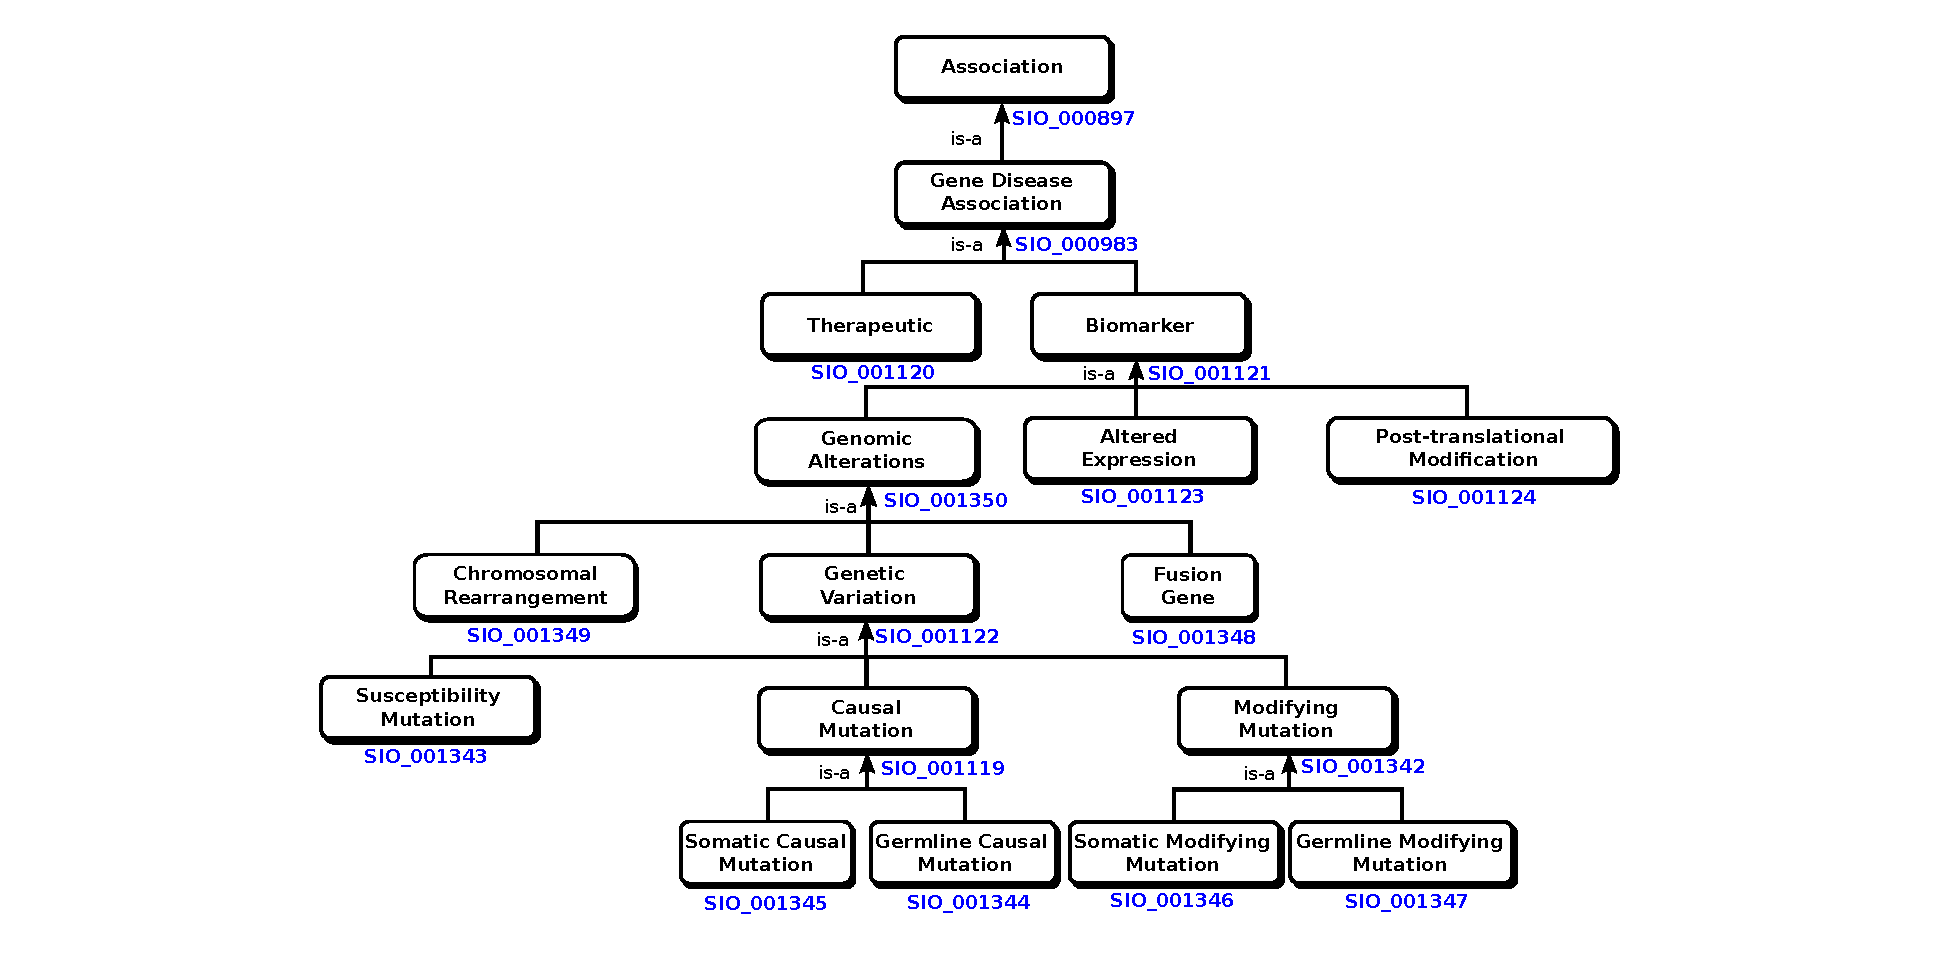
\includegraphics{pics/ontologyDisGeNET.pdf}}
    \caption{DisGeNET ontology \cite{DisGeNET2015}  \label{fig:disgenet_ontology}}
\end{figure}

Is not this similar to the already developed functional consequence score from Open Targets? It was obtained from \href{http://www.ontobee.org/ontology/SO?iri=http://purl.obolibrary.org/obo/SO_0001566}{OntoBee}

The labels from the original sources were mapped to DisGeNET Gene-Disease Ontology as detailed in Table \ref{tab:disgenet_ontology}.

\begin{table}[H]
    \centering
    \begin{tabular}{c|c}
    Association class & Original source label \\
    \hline
    
    \texttt{Altered Expression} & BeFree, LHGDN \\
    \texttt{Biomarker} & BeFree, HPO, LHGDN, MGD, PsyGeNET, RGD \\
    \texttt{Chromosomal Rearrangement} & Orphanet \\
    \texttt{Fusion Gene} & Orphanet \\
    \texttt{Genetic Variation} & BeFree, GAD, LHGDN, Orphanet, UniProt \\
    \texttt{Germline Causal Mutation} & Orphanet \\
    \texttt{Germline Modifying Mutation} & Orphanet \\
    \texttt{PostTranslational Modification} & BeFree, LHGDN \\
    \texttt{Somatic Causal Mutation} & Orphanet \\
    \texttt{Somatic Modifying Mutation} & Orphanet \\
    \texttt{Susceptibility Mutation} & ClinVar, Orphanet, RGD \\
    \texttt{Therapeutic} & CTD, RGD
    \end{tabular}
    \caption{Classification of the data sources into the \texttt{class nodes} in the DisGeNET ontology}
    \label{tab:disgenet_ontology}
\end{table}

% DISEASES
\newpage
\subsection{DISEASES}
\label{subsec:DISEASES}
\href{https://goo.gl/KGQsd9}{DISEASES} is a weekly updated web resource that integrates evidence on GDAs from (i) automatic text mining, (ii) manually curated literature, (iii) cancer mutation data, and (iv) GWAS \cite{DISEASES2015}. They further integrate all evidence data and define confidence scores that facilitate comparison of the different types and sources of evidence \cite{DISEASES2015}.

They use a Named Entity Recogniser (NER) that maps diseases in Medline abstracts to the \href{http://disease-ontology.org/}{Disease Ontology} \cite{schriml2012} in two processes: (i) namely recognition and (ii) normalization (also known as identification, mapping, or grounding).

\subsubsection{Data sources}
DISEASES integrates the GDAs extracted from automatic text mining with evidence from databases with permissive licenses, namely manually curated associations (see Table \ref{tab:diseases_data}).
\begin{table}[H]
\centering
    \begin{tabular}{c|c}
         Source & Description  \\
         \hline
         \href{https://goo.gl/gnQSYt}{GHR} & Genetic variation and diseases at NIH*\\
         \href{https://goo.gl/d2PhpC}{UniProtKB} & Curated protein functional data \cite{uniprot2017} \\
         \href{https://goo.gl/hYjVeR}{DistiLD} & GWAS linked to ICD-10 codes \cite{palleja2011} \\
         \href{https://goo.gl/qcY8qo}{COSMIC} & Somatic mutation cancer data \cite{cosmic2017}
    \end{tabular}
    \caption{Data sources used by DISEASES \cite{DISEASES2015} \label{tab:diseases_data}}
\end{table}
* GHR does not provide download files. DISEASES used an automated crawler algorithm to download the web page for each disease and store the disease name, which is part of the uniform resource locator (URL), along with any gene symbols listed on the web page \cite{DISEASES2015}.

% Open Targets
\newpage
\subsection{Open Targets}
\label{subsec:ot}

Open Targets is a large--scale, public--private partnership with the aim of generating an informatics platform that utilises genetic germline, genetic somatic, gene expression, literature, pathway, and drug data to link 18,104 genes and diseases, with the ultimate objective of developing a systematic priorisation of gene--disease associations (GDAs) \cite{ferrero2017}.
\begin{itemize}
    \item Which were the \textbf{targets}? The targets could be a genes, transcripts or proteins defined by standard nomenclature. Which one is this nomenclature? Ensembl? HUGO? I think it is Ensembl for their research
    
    \item Which were the \textbf{diseases}? Diseases were described by the \href{https://goo.gl/YvvC8D}{EFO} \cite{experimentalFactorOntology2010}
    
    \item How they relate phenotypes to diseases? The evidence is described in the \href{https://goo.gl/CNqAqt}{Open Biomedical AssociatioN} (OBAN) representation \cite{sarntivijai2016}. OBAN is an ontology that represents triple-form entities of \texttt{subject--related--to\_object}. For example, an entity \texttt{disease} is the subject, the relationship \texttt{has\_evidence} and the objects could be entities \texttt{phenotypes} plus the source of evidence for that association
    
\end{itemize}

\subsubsection{Data sources}
\label{subsubsec:ot_ds}
% Always in this alphabetic order:
% Affected pathway
% Animal model
% Genetic association
% Somatic association
% Known drug
% Literature text mining
% RNA expression

The information obtained from different public domain databases (see Table \ref{tab:ot_db}) was classified into seven different \texttt{data types}:

\begin{itemize}
    \item \texttt{affected\_pathway}: if the gene is known to be part of a pathway that is affected in disease

    \item \texttt{animal\_model}: if an animal model with a gene knockout or phenotype that manifests in phenotype concordant with human disease
    
    \item \texttt{genetic\_association}: if there are germline mutation with either common disease primarily from GWAS or rare Mendelian disease from sequencing of exons of protein coding genes
    
    \item \texttt{somatic\_association}: if there is somatic mutation in the gene associated with the disease
    
    \item \texttt{known\_drug}: if there is an existing drug that engages the target and is used to treat the disease from \href{https://goo.gl/tJ2wzt}{ChEMBL}
    
    \item \texttt{literature} if a GDA was identified through co-occurrence in full text articles from \href{https://europepmc.org/}{Europe PMC database} \cite{koscielny2016}
    
    \item \texttt{rna\_expression}: if there are significant gene expression changes in appropriate sample comparisons from microarray or RNA-seq experiments as a consequence of the disease
\end{itemize}

\begin{table}[H]
\centering
    \begin{tabular}{c|c|c|c}
      Data source & Data type & \texttt{evidence\_score} \\
      \hline
      
      \href{https://goo.gl/sfm7CC}{Reactome} & Affected pathway &
      Curator score = \{1,0\} \\
      
      \href{https://goo.gl/egMxCH}{PhenoDigm} & Animal Model &
      Similarity score \cite{PhenoDigm2013} \\
      
      \href{https://goo.gl/A4UjA5}{GWAS Catalog} & Genetic association &
      $ FCS^* \cdot sample\_size \cdot p_{value} $ \\
      
      \href{https://goo.gl/Vavb1L}{EVA} & Genetic association & 
      FCS* \\
      
      \href{https://goo.gl/5SiDMj}{UniProt} & Genetic association &
      Curator score = \{0.5,1\} \\
      
      \href{https://goo.gl/qwDPhK}{Gene2Phenotype} & Genetic association &
      Curator score = 1 \\
      
      \href{https://goo.gl/dXL3jQ}{Cancer Gene Census} & Somatic mutation &
      FCS* \\
      
      \href{https://goo.gl/kTWn6z}{IntOGen} & Somatic Mutation &
      Tumor type category score = \{0.25, 0.5, 0.75\}\\
      
      \href{https://goo.gl/tJ2wzt}{ChEMBL} & Known drug & Clinical phase score = \{0.09, 0.1, 0.2, 0.7, 1.0\} \\
      
      \href{https://goo.gl/P3UAc9}{Europe PMC} & Literature text mining & Confidence score \cite{kafkas2017} \\
      
      \href{https://goo.gl/1eQbbs}{Gene Expression Atlas} & RNA expression & $p_{value} \cdot sample\_size \cdot percentile\_rank $ \\
      
      \end{tabular}
\caption{Data sources for GDA information the Open Targets pipeline. The \texttt{evidence\_score} is described in Section \ref{subsubsec:ot_scores}. A more detailed explanation of the \texttt{evidence\_score} is described by Koscielny et al. \cite{koscielny2016} \label{tab:ot_db}}
\end{table}

* FCS means Functional Consequence Score. Available in \href{https://goo.gl/gkvHxK}{Supplementary Table 2. Functional consequence score}

All information in Open Targets is stored in JSON format. An example of the JSON format they use can be viewed in Figure \ref{fig:ot_json}.

\begin{figure}[H]
    \centering
    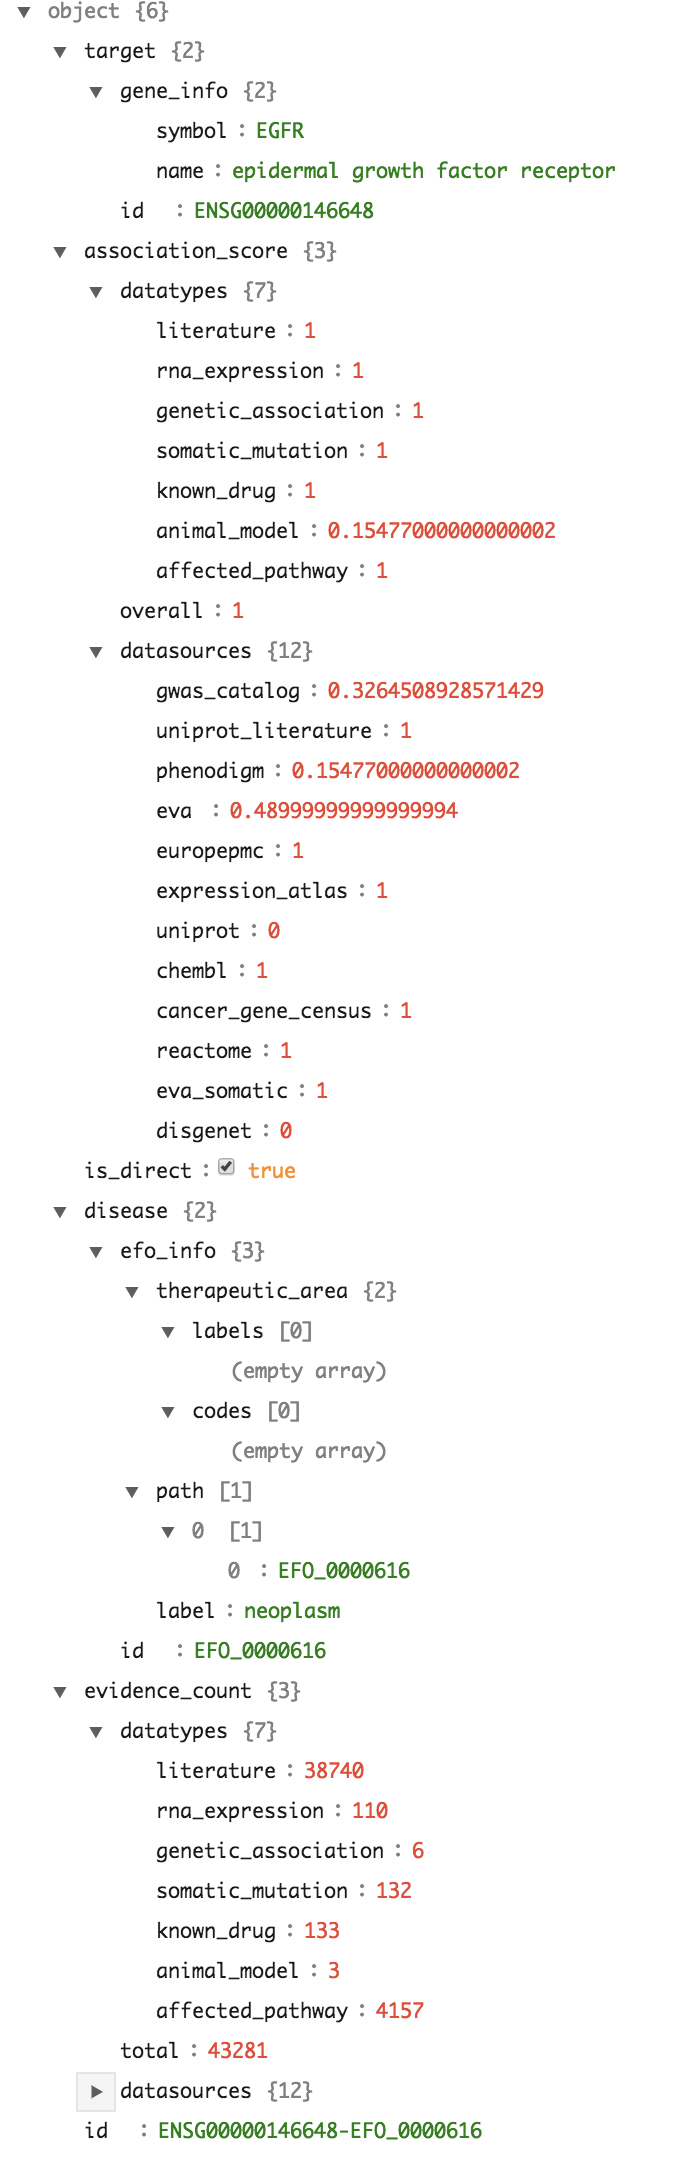
\includegraphics[width=7cm]{pics/ot_json.png}
    \caption{JSON format in Open Targets \label{fig:ot_json}}
\end{figure}

\subsubsection{Scores}
\label{subsubsec:ot_scores}

\begin{itemize}
    \item \texttt{evidence\_score} that attempts to comprise the (i) \texttt{frequency}, (ii) \texttt{magnitude}, and (iii) \texttt{confidence} of GDAs \cite{koscielny2016} in Table \ref{tab:ot_db}. E.g. in a GWAS evidence from GWAS Catalog: the \texttt{frequency} is the sample size, the \texttt{magnitude} is the predicted functional consequence of the variation, and the \texttt{confidence} is the p-value
    
    \item \texttt{data\_source\_score} defined as the \emph{harmonic sum} of all sorted evidence scores in descending order. E.g. in a GWAS evidence from GWAS Catalog: all \texttt{evidence scores} are sorted in descending order and the \texttt{data\_source\_score} is calculated based on the formula below:
    
    $$ S_{1,...i} = S_1 + \frac{S_2}{2^2} + \frac{S_3}{3^2} + ... + \frac{S_i}{i^2}$$
    
    \item \texttt{data\_type\_score} follows a similar approach to the \texttt{data\_source\_score}. It uses the \emph{harmonic sum} to derive a unique score for each of the data types described in Section \ref{subsubsec:ot_ds}. E.g. in a GWAS evidence, the harmonic sum is calculated based on the formula above with the four \texttt{data\_source\_scores} for \texttt{genetic\_association}: GWAS Catalog, EVA, UniProt, and Gene2Phenotype in Table \ref{tab:ot_db}
    
    
    
    \item \texttt{overall\_score} follows the same approach as the \texttt{data\_type\_score} and \texttt{data\_source\_score}
\end{itemize}

Why the harmonic sum? Is there a better score? Idea: use different scores and do a sensitivity analysis

Why they include \texttt{sample\_size}? It is already included in the p-value! The p-value is a measure of uncertainty. The more data, the less uncertainty. The code snippet below in \texttt{Python} will demonstrate it:

\lstinputlisting[language=Python]{data/pval_uncertainty.py}

\subsubsection{Reproduction of pipeline}
Ferrero et al. code in R version 3.3.0 was versioned using GitHub and is available \href{https://goo.gl/C4cSgQ}{elsewhere}.
They defined different sets in the workflow (see Figure \ref{fig:ot_workflow}):
\begin{itemize}
    \item The \texttt{main set} (2016 Apr version) is a \texttt{JSON} file downloaded from the \href{https://goo.gl/BdqKkH}{platform download page} and contains all Open Targets GDAs. Just 5 of the 7 described features in Section \ref{subsubsec:ot_ds} were used: \texttt{affected\_pathway}, \texttt{animal\_model}, \texttt{genetic\_association}, \texttt{rna\_expression} and \texttt{somatic\_mutation}. They removed \texttt{known\_drug} and \texttt{literature}
    
    \item The \texttt{label set} with information on (i) genes and (ii) associated drugs based on PharmaProjects data \cite{pharmaProjects}. Genes with drugs in Preclinical, Clinical Trial Phase I, Clinical Trial Phase II, Clinical Trial Phase III, Pre-registration, Registered, or Launched were considered targets. Failed and Abandoned drugs were ignored. \textbf{Important} The results in this report were obtained using the targets from Cortellis, provided by Guillermo.
    
    \item The \texttt{working set} with all known PharmaProject targets (n=1421) and randomly selected unlabelled (n=1421)
    
    \item The \texttt{prediction set} with the remaining unlabelled genes (n=15262) that was set aside for the prediction of targets
\end{itemize}

Restrictions apply to the availability of the Pharmaprojects data \cite{ferrero2017}. Why did Open Targets used PharmaProjects data if they had \href{https://goo.gl/StJTq2}{ChEMBL} \cite{chembl2014} data as mentioned in Section \ref{subsubsec:ot_ds}?
\begin{itemize}
    \item It covers early stage announcements
    \item It contains more targets with drug annotations (2105 versus 625)
    \item It discriminates between drug development phases: Preclinical, Clinical Trial, Phase I Clinical Trial, Phase II Clinical Trial, Phase III Clinical Trial, Pre-registration, Registered, Launched, Failed, or Abandoned
\end{itemize}


\begin{figure}[H]
    \centering
    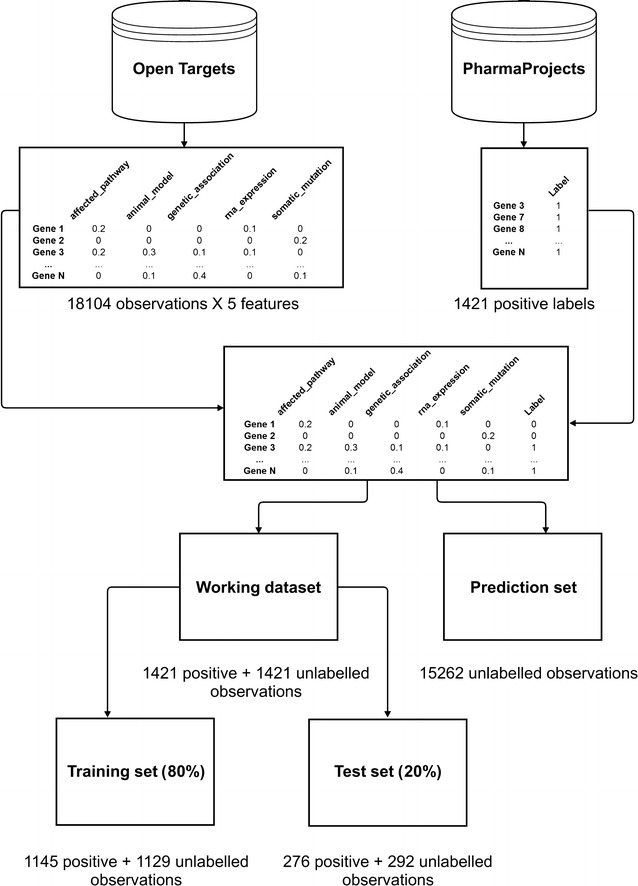
\includegraphics[width=0.7\textwidth]{pics/workflowOpenTargets.jpg}
    \caption{Explanatory workflow for the prediction of therapeutic targets based on GDAs. Observations and features were gathered by Open Targets based on just 5 of the 7 data types from Section \ref{subsubsec:ot_ds} while the labels were collected from Informa Pharmaprojects \cite{pharmaProjects} (my results use Cortellis targets provided by Guillermo). The resulting data matrix was split into a \texttt{working set} (1421 positives and 1421 randomly selected unlabelled) and a \texttt{prediction set} (15262 unlabelled genes). The \texttt{working set}, containing both positive and unlabelled observations, was further split into \texttt{training set} and \texttt{test set} to evaluate the performance of the classifier. The \texttt{prediction set} was kept aside and used to perform predictions once all four classifiers was trained}
    \label{fig:ot_workflow}
\end{figure}

Second, Ferrero et al. \cite{ferrero2017} carried out an exploratory analysis on the \texttt{working set} using two unsupervised methods: principal component analysis (PCA) and t-Stochastic Neighbourhood Embedding (tSNE). PCA and t-SNE results are displayed in Figure \ref{fig:OT_PCA} and Figure \ref{fig:OT_tSNE} respectively.

\begin{figure}[H]
\resizebox{\textwidth}{!}{
    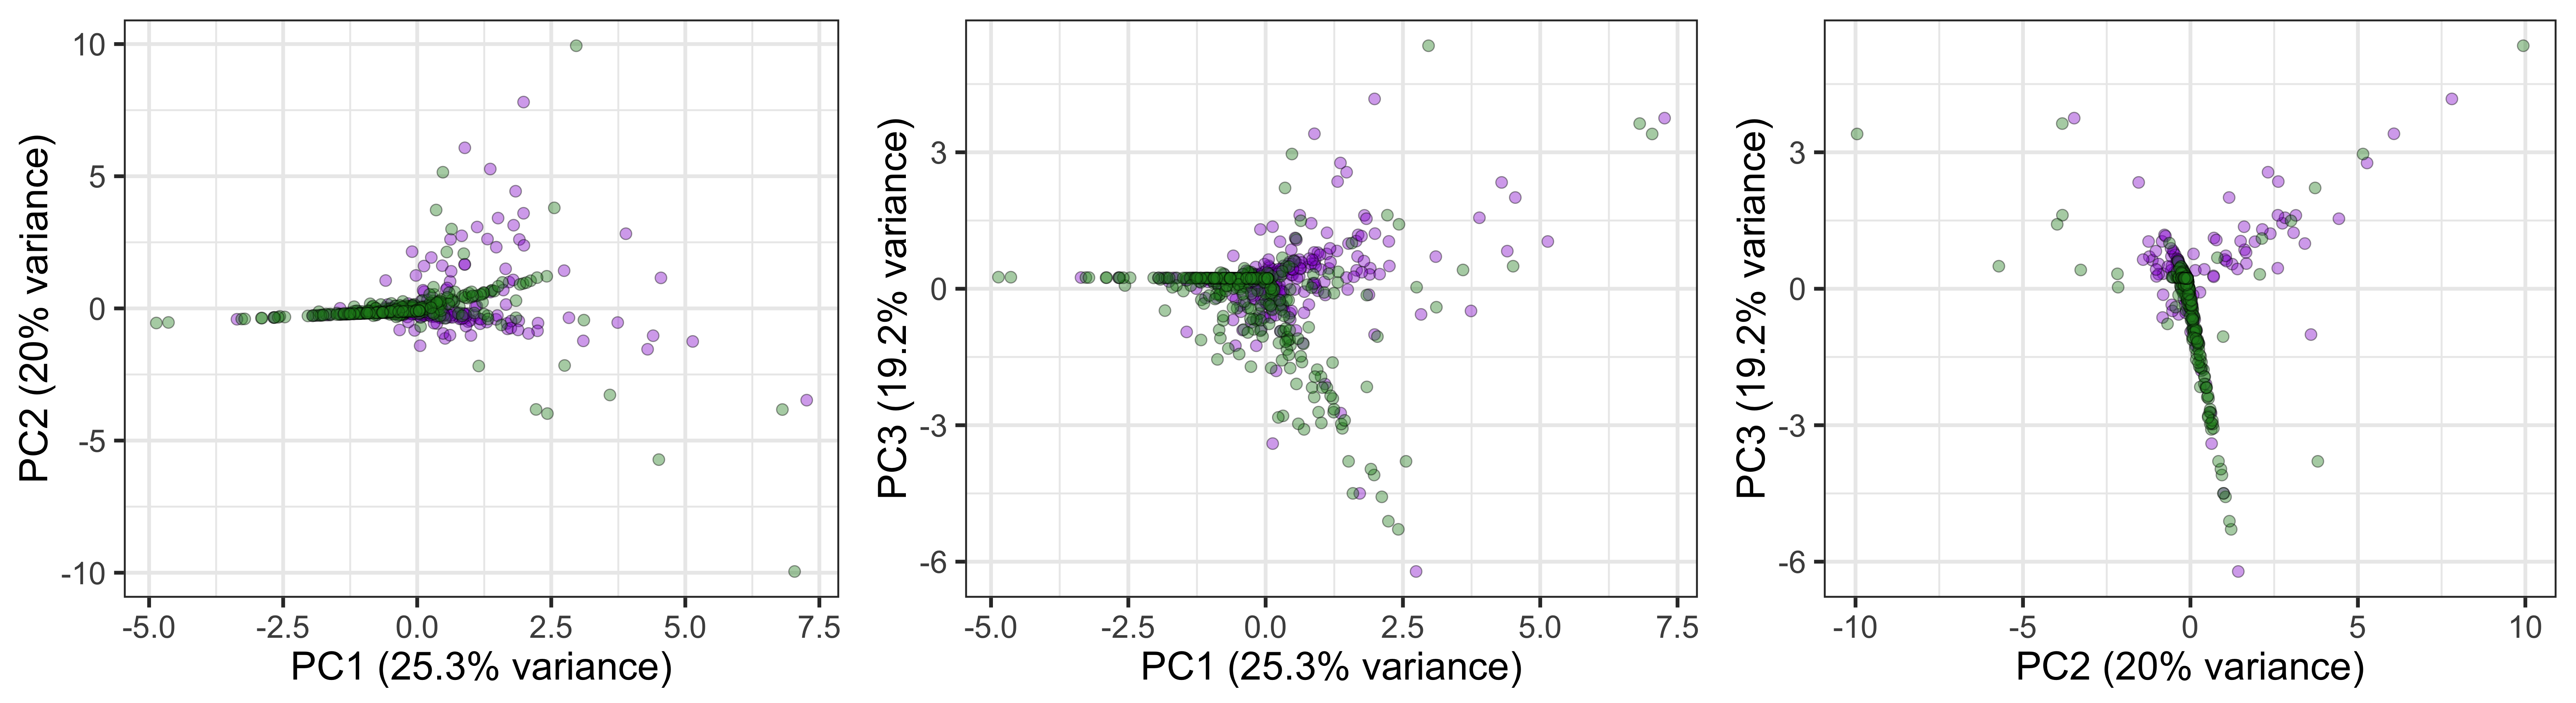
\includegraphics{pics/PCAh.png}}
    \caption{Exploratory data analysis of the \texttt{working set} using PCA for linear dimensionality reduction. Each dot in the two-dimensional space represents a gene and is coloured according to its label (green target, purple non-target)}
    \label{fig:OT_PCA}
\end{figure}

\begin{figure}[H]
\centering
    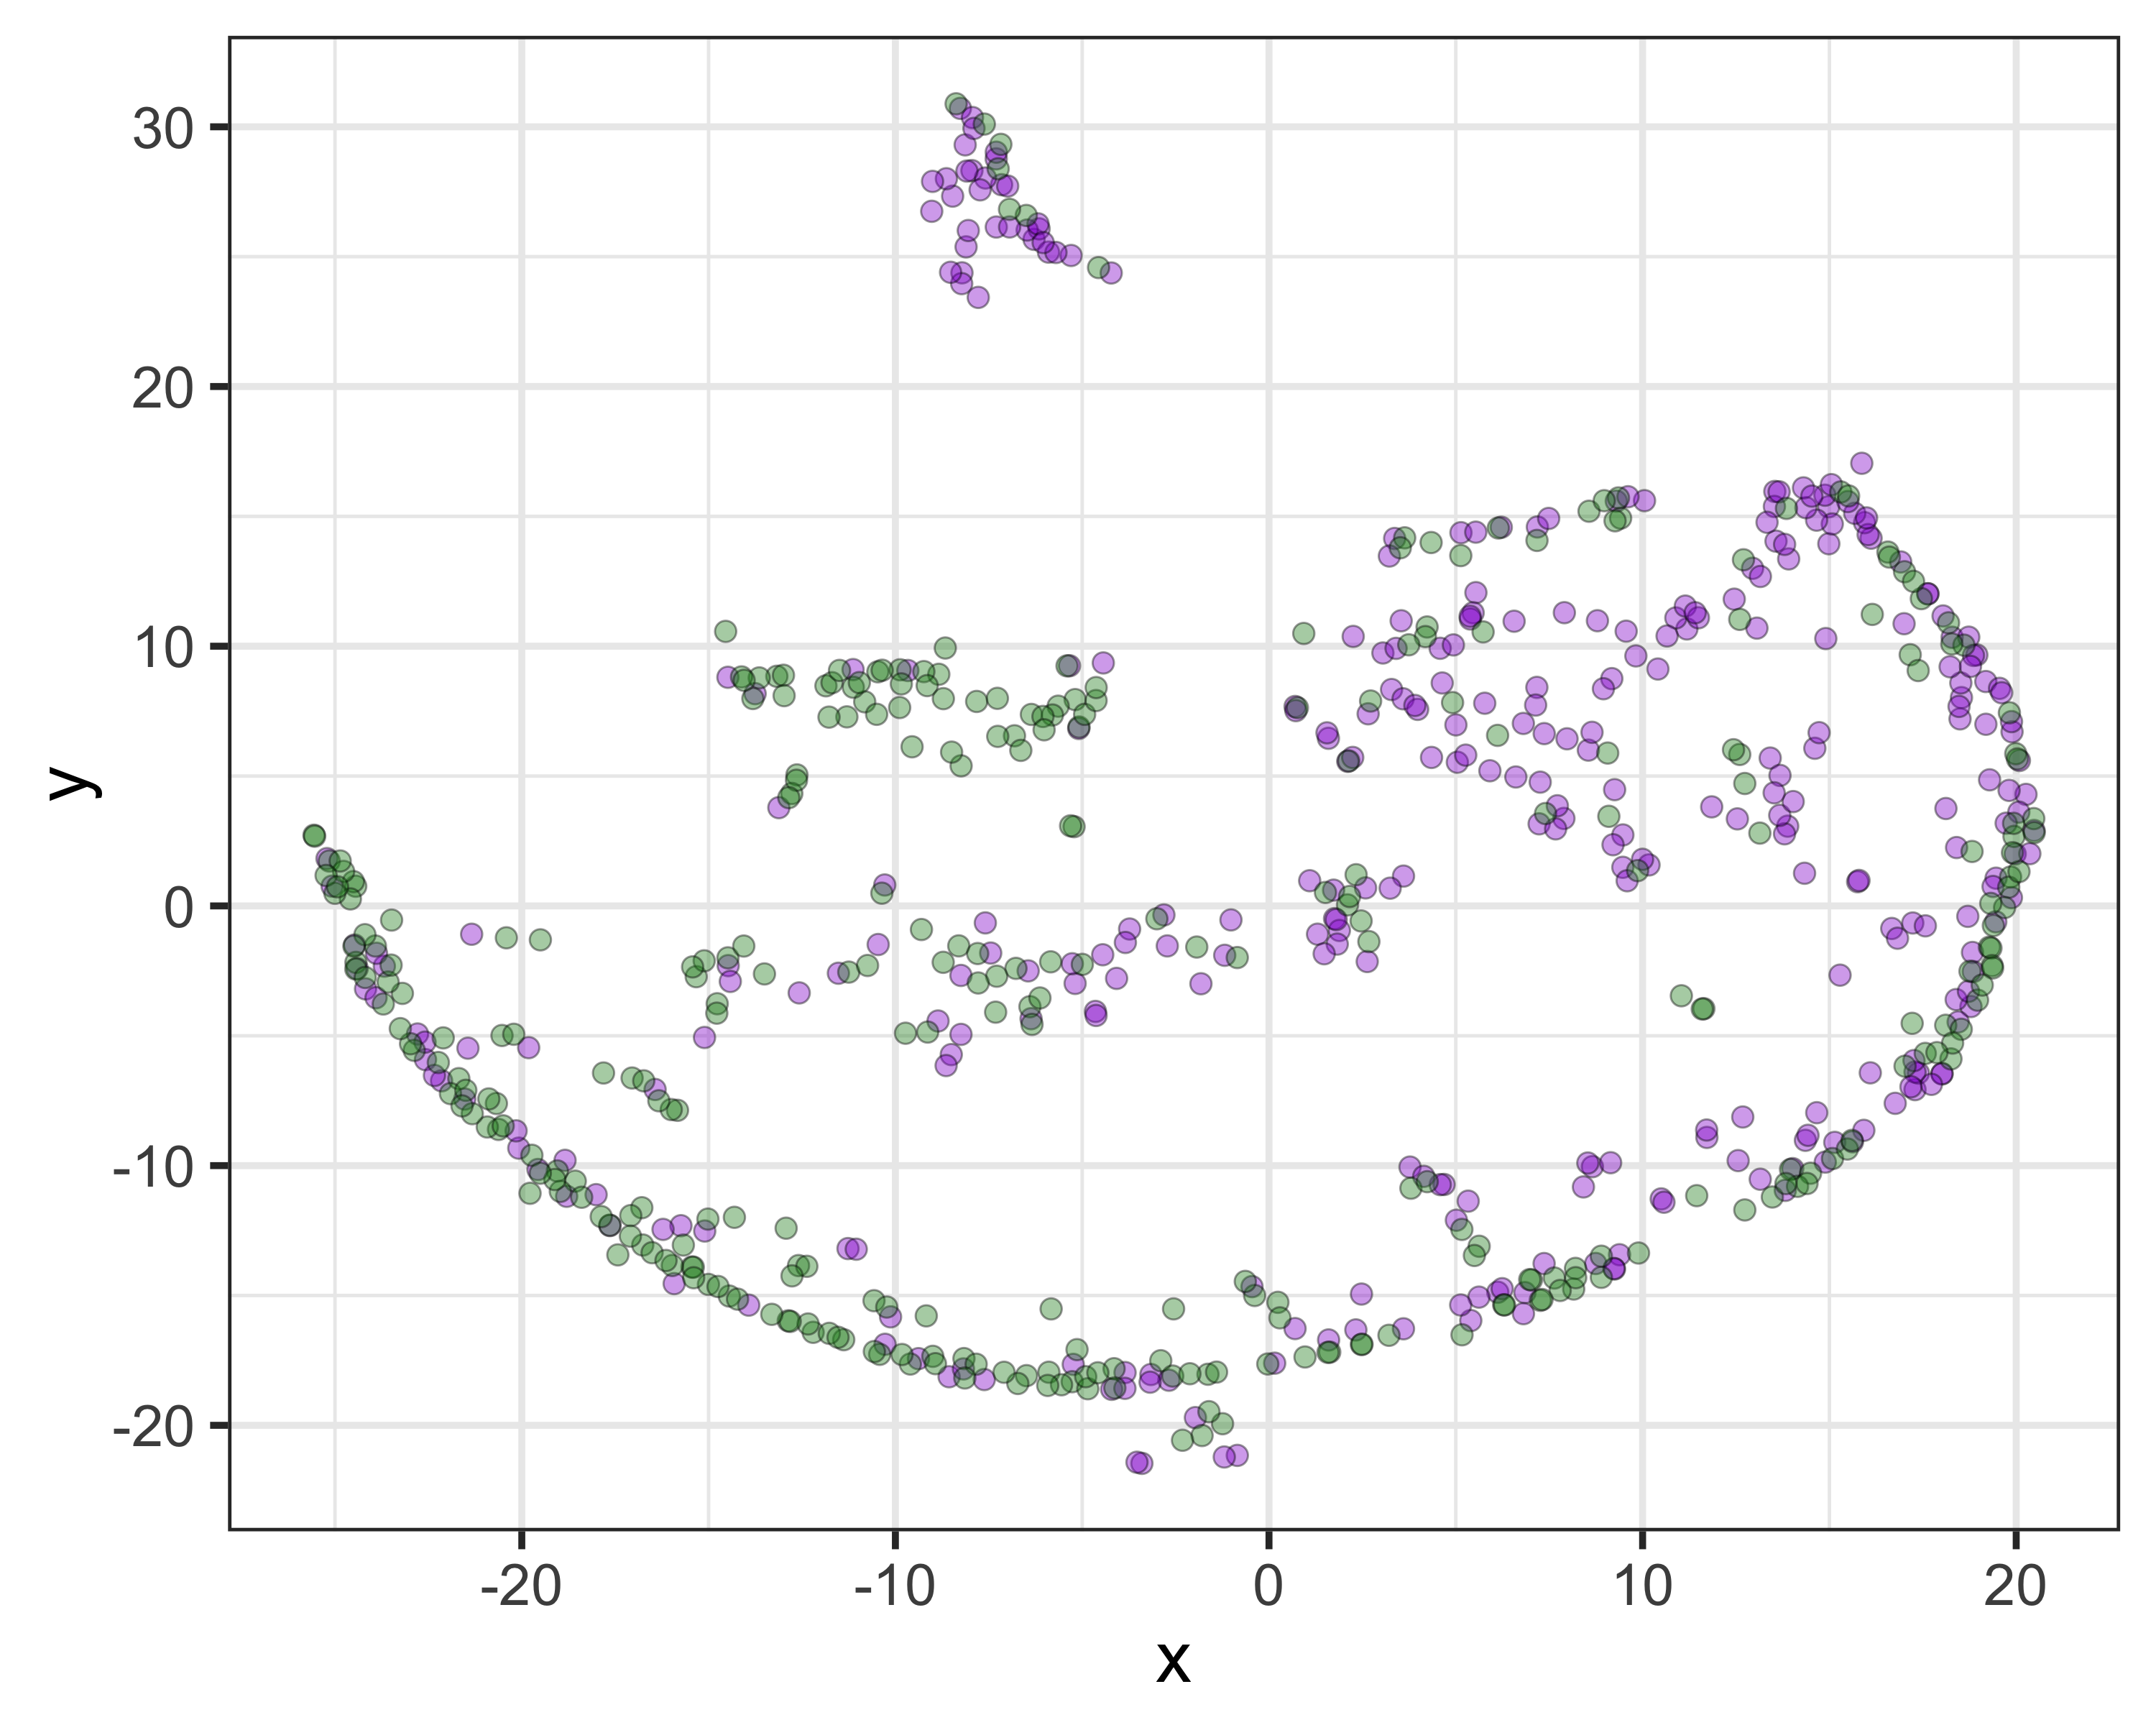
\includegraphics[width=11cm]{pics/tSNE.png}
    \caption{Exploratory data analysis of the \texttt{working set} using dimensionality reduction. The tSNE algorithm for non-linear dimensionality reduction was run a perplexity value of 30 and other default parameters. Each dot in the two-dimensional space represents a gene and is coloured according to its label (green target, purple non-target)}
    \label{fig:OT_tSNE}
\end{figure}

tSNE resulted in a rather clear separation between targets and non-targets on a two-dimensional space (see Figure \ref{fig:OT_tSNE}: most of the data points labelled as targets lie on a curved line and a gradient of targets and non-targets is present along the vertical axis. This results are clearly similar to Ferrero et al. \cite{ferrero2017}, showing that there is a distinction between therapeutic targets and non-targets in Open Targets data.

Next, they investigated the contributions of all five individual data types and their relative importance in the \texttt{working set} with two methods: (i) Chi squared test and (ii) information gaining in Figure \ref{fig:OT_features}. \texttt{animal\_model}, \texttt{rna\_expression} and \texttt{genetic\_association} showed the highest values and association with the outcome binary variable in both their and my results (see Figure \ref{fig:OT_features}).

\begin{figure}[H]
\centering
    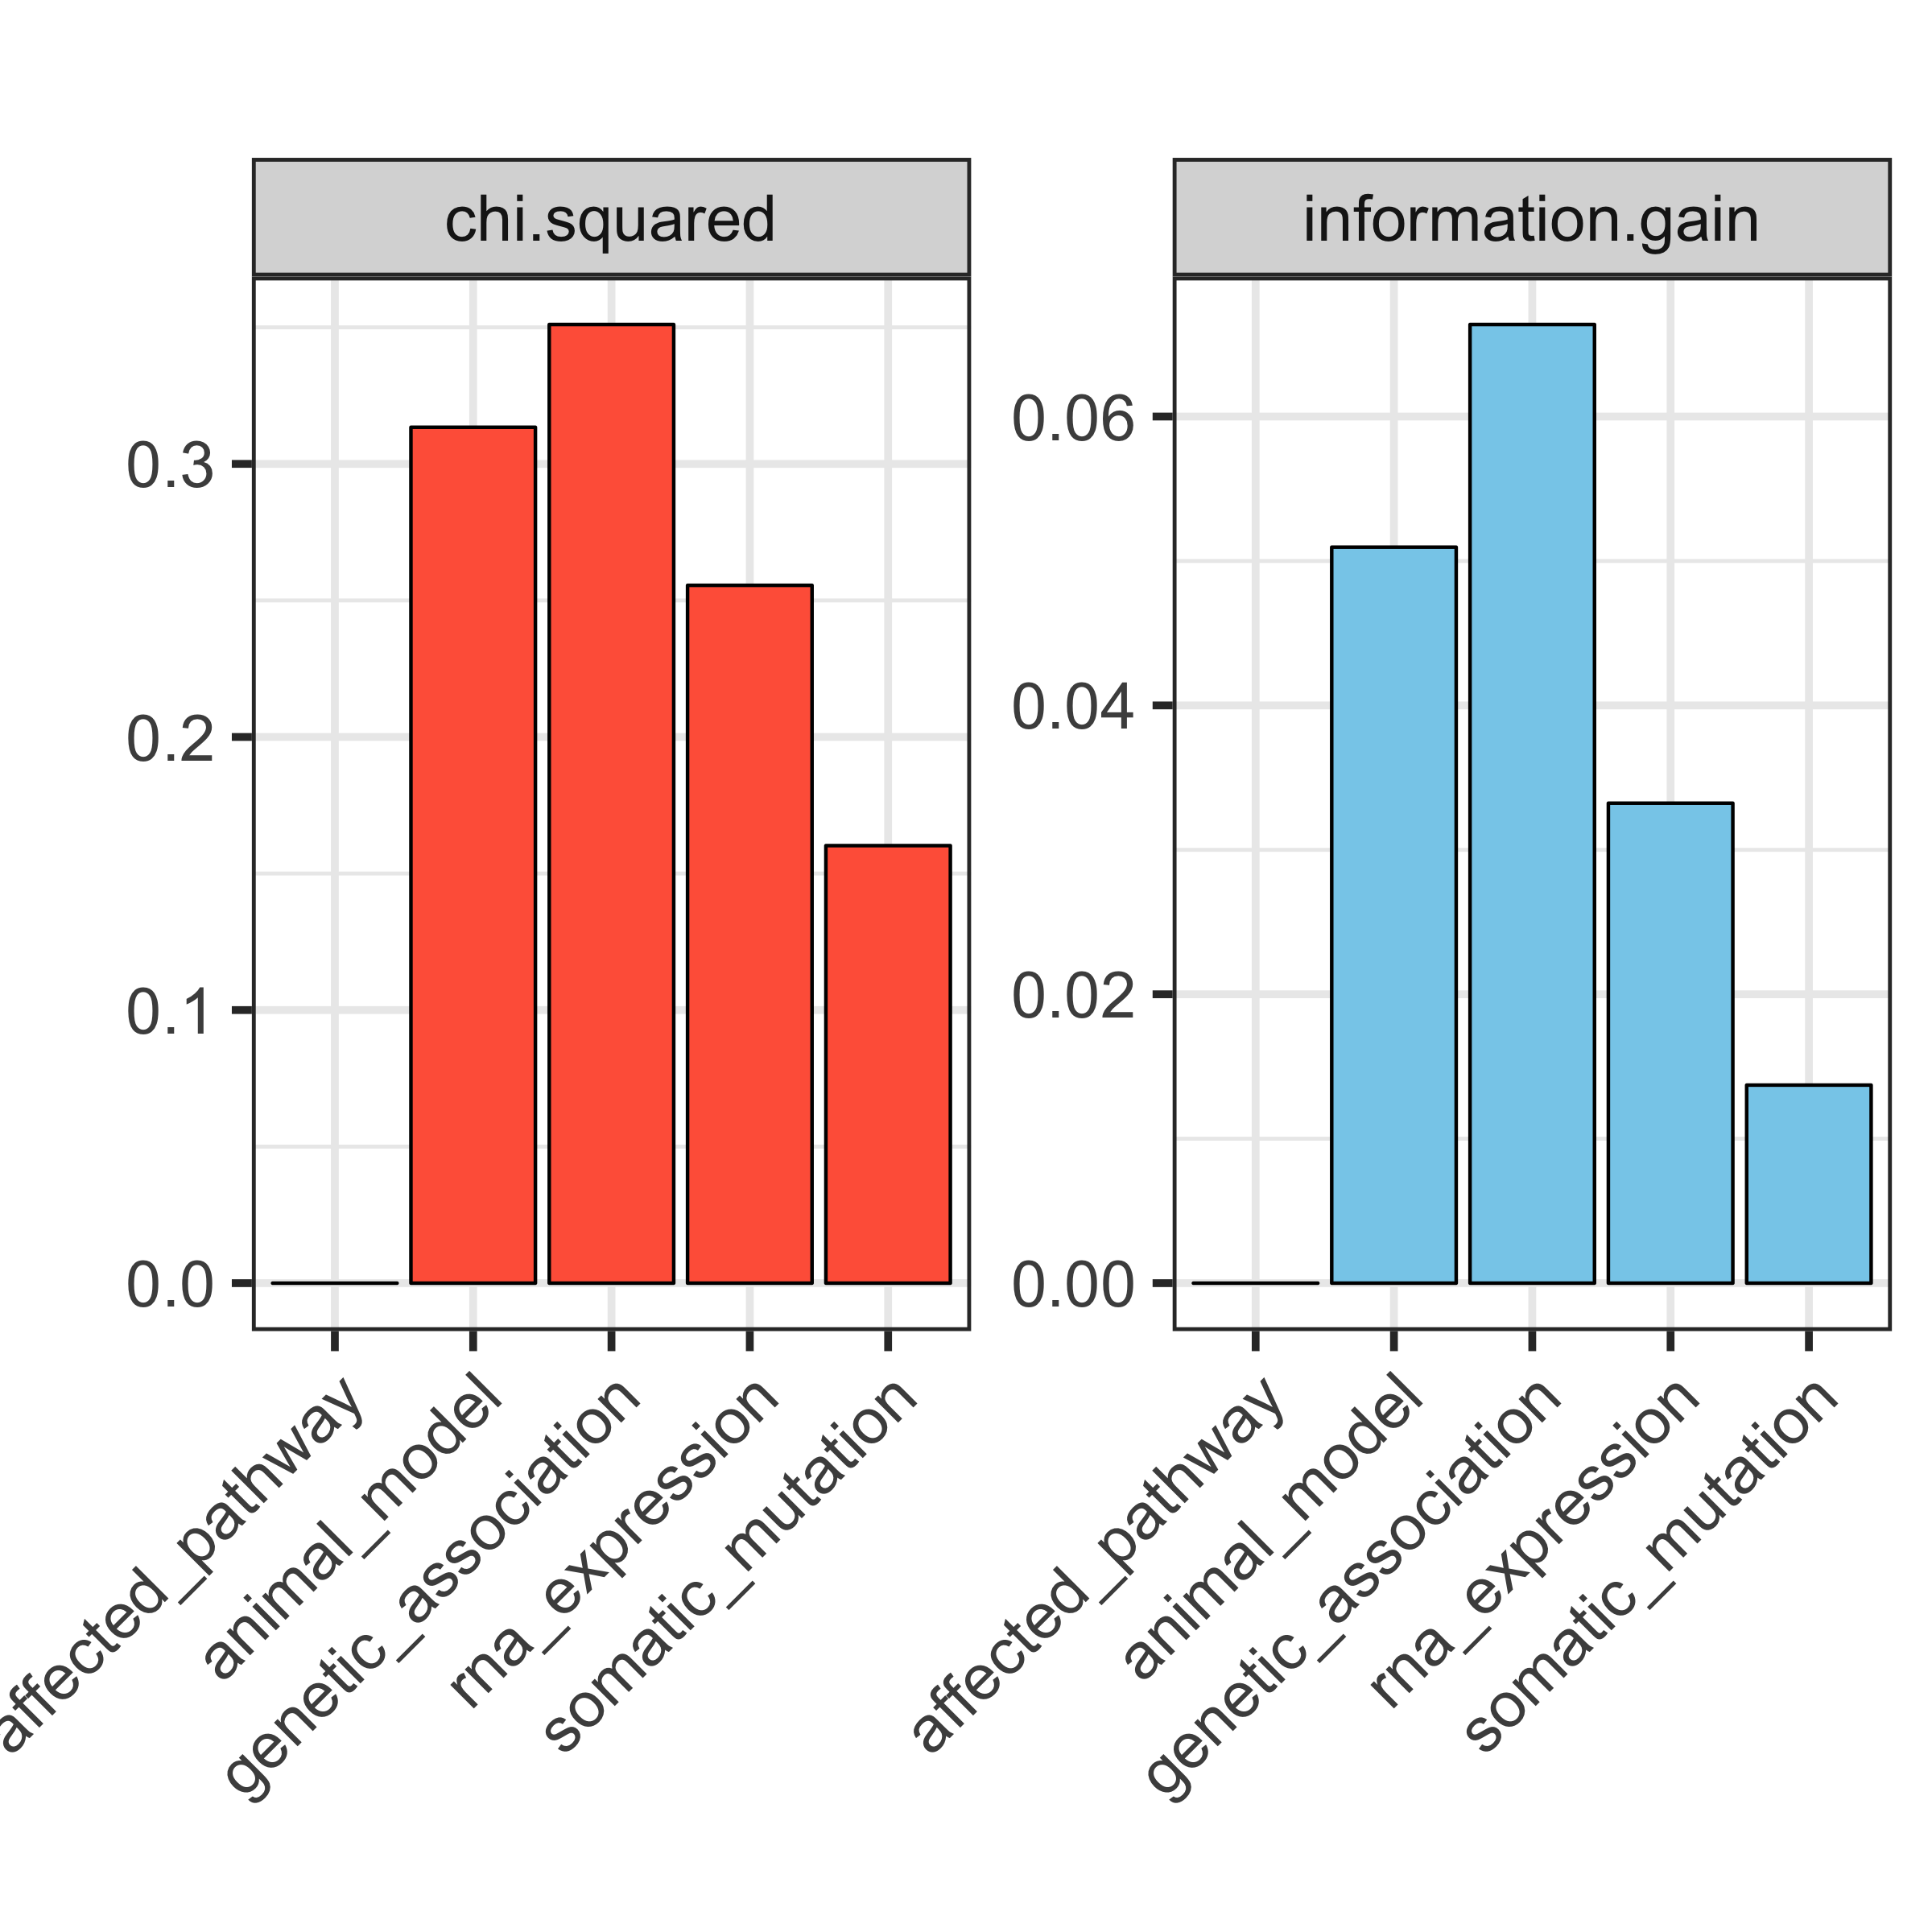
\includegraphics[width=7cm]{pics/Features.png}
    \caption{Feature importance according to two independent feature selection methods (left to right): Chi squared test and information gain with the \texttt{working set}}
    \label{fig:OT_features}
\end{figure}

They explored the classification criteria of a decision tree model to get insights into the best features for classification. Again, \texttt{animal\_model}, \texttt{rna\_expression} and \texttt{genetic\_association} were the most important features for target classification. These results are important and will be discussed in Section \ref{subsub:limitations_openTargets}.

\begin{figure}[H]
    \centering
    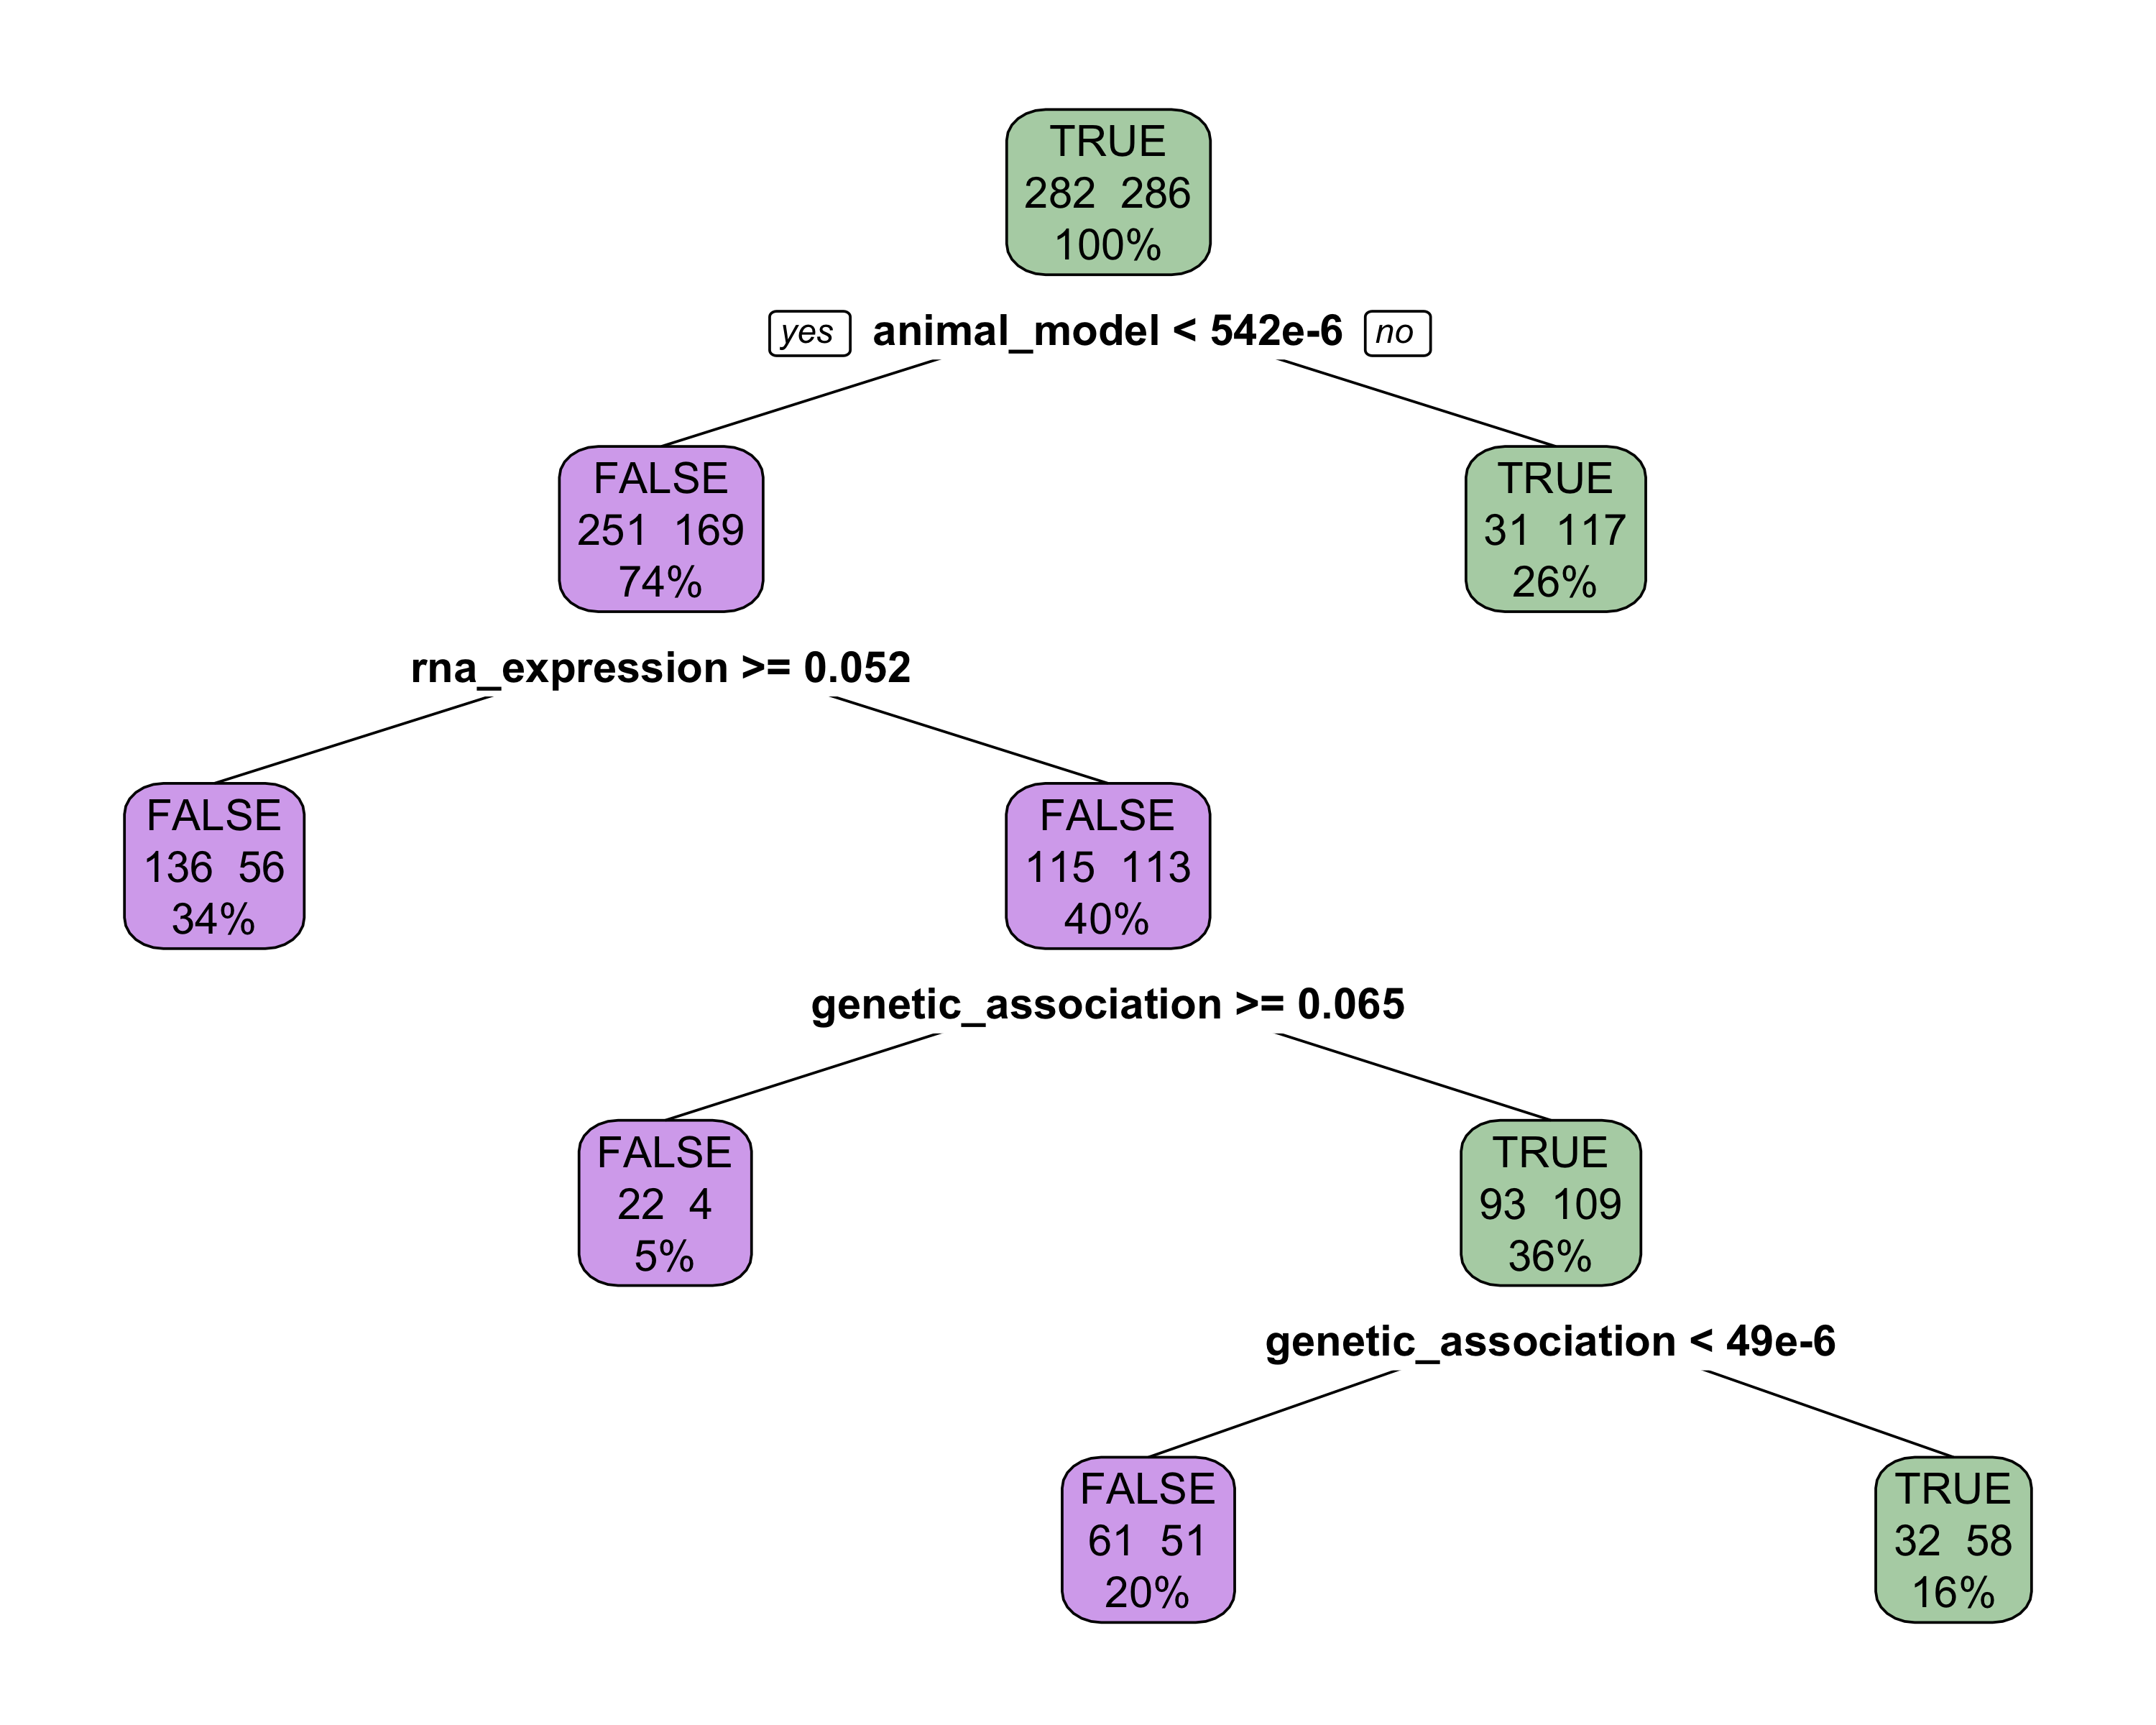
\includegraphics[width=11cm]{pics/DecisionTreeInf.png}
    \caption{Decision tree classification criteria: colours represent predicted outcome (purple non-target, green target). In each node, numbers represent (from top to bottom): outcome (FALSE: non-target, TRUE: target), number of observations in node per class (left non-target, right target), percentage of observations in node}
    \label{fig:OT_decisionTree}
\end{figure}

Open Targets used a (i) \emph{semi-supervised} approach on (ii) \emph{positive} and unlabelled data with (iii) nested cross-validation (NCV) to know if their GDAs could contain relevant information to binary classify therapeutic targets \cite{ferrero2017} according to PharmaProjects data \cite{pharmaProjects}. This aim is very important and will be discussed in \ref{subsub:limitations_openTargets}. Ferrero et al. used four different ML binary classifiers:
\begin{itemize}
    \item \textbf{Random Forest} (RF)
    \item \textbf{Support Vector Machine} (SVM) with a radial kernel
    \item Feed-forward \textbf{Neural Network} (NN) with a single hidden unit
    \item \textbf{Gradient Boosting Machine} (GBM) using the \emph{AdaBoost} exponential loss function
\end{itemize}

Why \textbf{semi-supervised}? Because the data was partially labelled. Out of the 18,104 genes, just 1,421 genes were known to be related to drugs with information about their current development phase: Preclinical, Clinical Trial, Phase I Clinical Trial, Phase II Clinical Trial, Phase III Clinical Trial, Pre-registration, Registered, Launched, (Failed, or Abandoned? this will be negative labelling) according to Informa Pharmaprojects data \cite{pharmaProjects}. Restrictions apply to the availability of the Pharmaprojects data, which was used under license for the current study, and so is not publicly available \cite{ferrero2017}. Failed or abandoned projects according to Pharmaprojects were ignored \cite{ferrero2017}. It is uncertain whether the remaining 16,683 genes may become a potential target in the future \cite{ferrero2017}. Semi-supervised methods tackle problems where there is a mixture of labelled and unlabelled data.
    
Why \textbf{positive} labelled? Because all genes known to be related to drugs are the ones that are in any of the above categories, labelled as belonging to an active or \emph{positive} drug discovery process. This type of problem is known as Positive-Unlabelled or PU learning. To account for this problem, bootstrap aggregating (\emph{bagging}) with 100 iterations was applied to the SVM, the NN and the GBM classifiers. RF does \emph{bagging} by default in R 3.3.0
    
Why \textbf{nested cross-validation} (NCV)? Because NCV generalises the estimation error of the model and its hyperparameters in an inner loop. Non-NCV biases the model yielding an overly optimistic score. A comparison between NCV and non-NCV in Python can be found \href{https://goo.gl/soHYT7}{elsewhere}. Ferrero et al. used NCV with a 4-fold inner loop to optimise the hyperparameters and a 4-fold outer loop to estimate the performance in the \texttt{training set}. \emph{Hyperparameters} are parameters that are intrinsic to the defined model and are set prior to the training process. The \emph{parameters} of the model are derived from the ML training process. With NCV there is a inner loop to search for the best hyperparameters and, secondly, an outer loop to optimise the parameters.


Different measures were used to assess the classifiers (RF, SVM, NN and GBM):
\begin{itemize}
    \item Receiver operating characteristic (ROC) curves in Figure \ref{fig:OT_ROC}
    \item Precision-recall curves in Figure \ref{fig:OT_precisionRecall}
    \item Misclassification errors in Figure \ref{fig:OT_MmceBoxplots}
    \item Box plots for the distribution of the following measures: area under the curve (AUC), accuracy, F1 measure, precision, recall/sensitivity ratio, and specificity in Figure \ref{fig:OT_OtherPlots}
\end{itemize}

\begin{figure}[H]
    \centering
    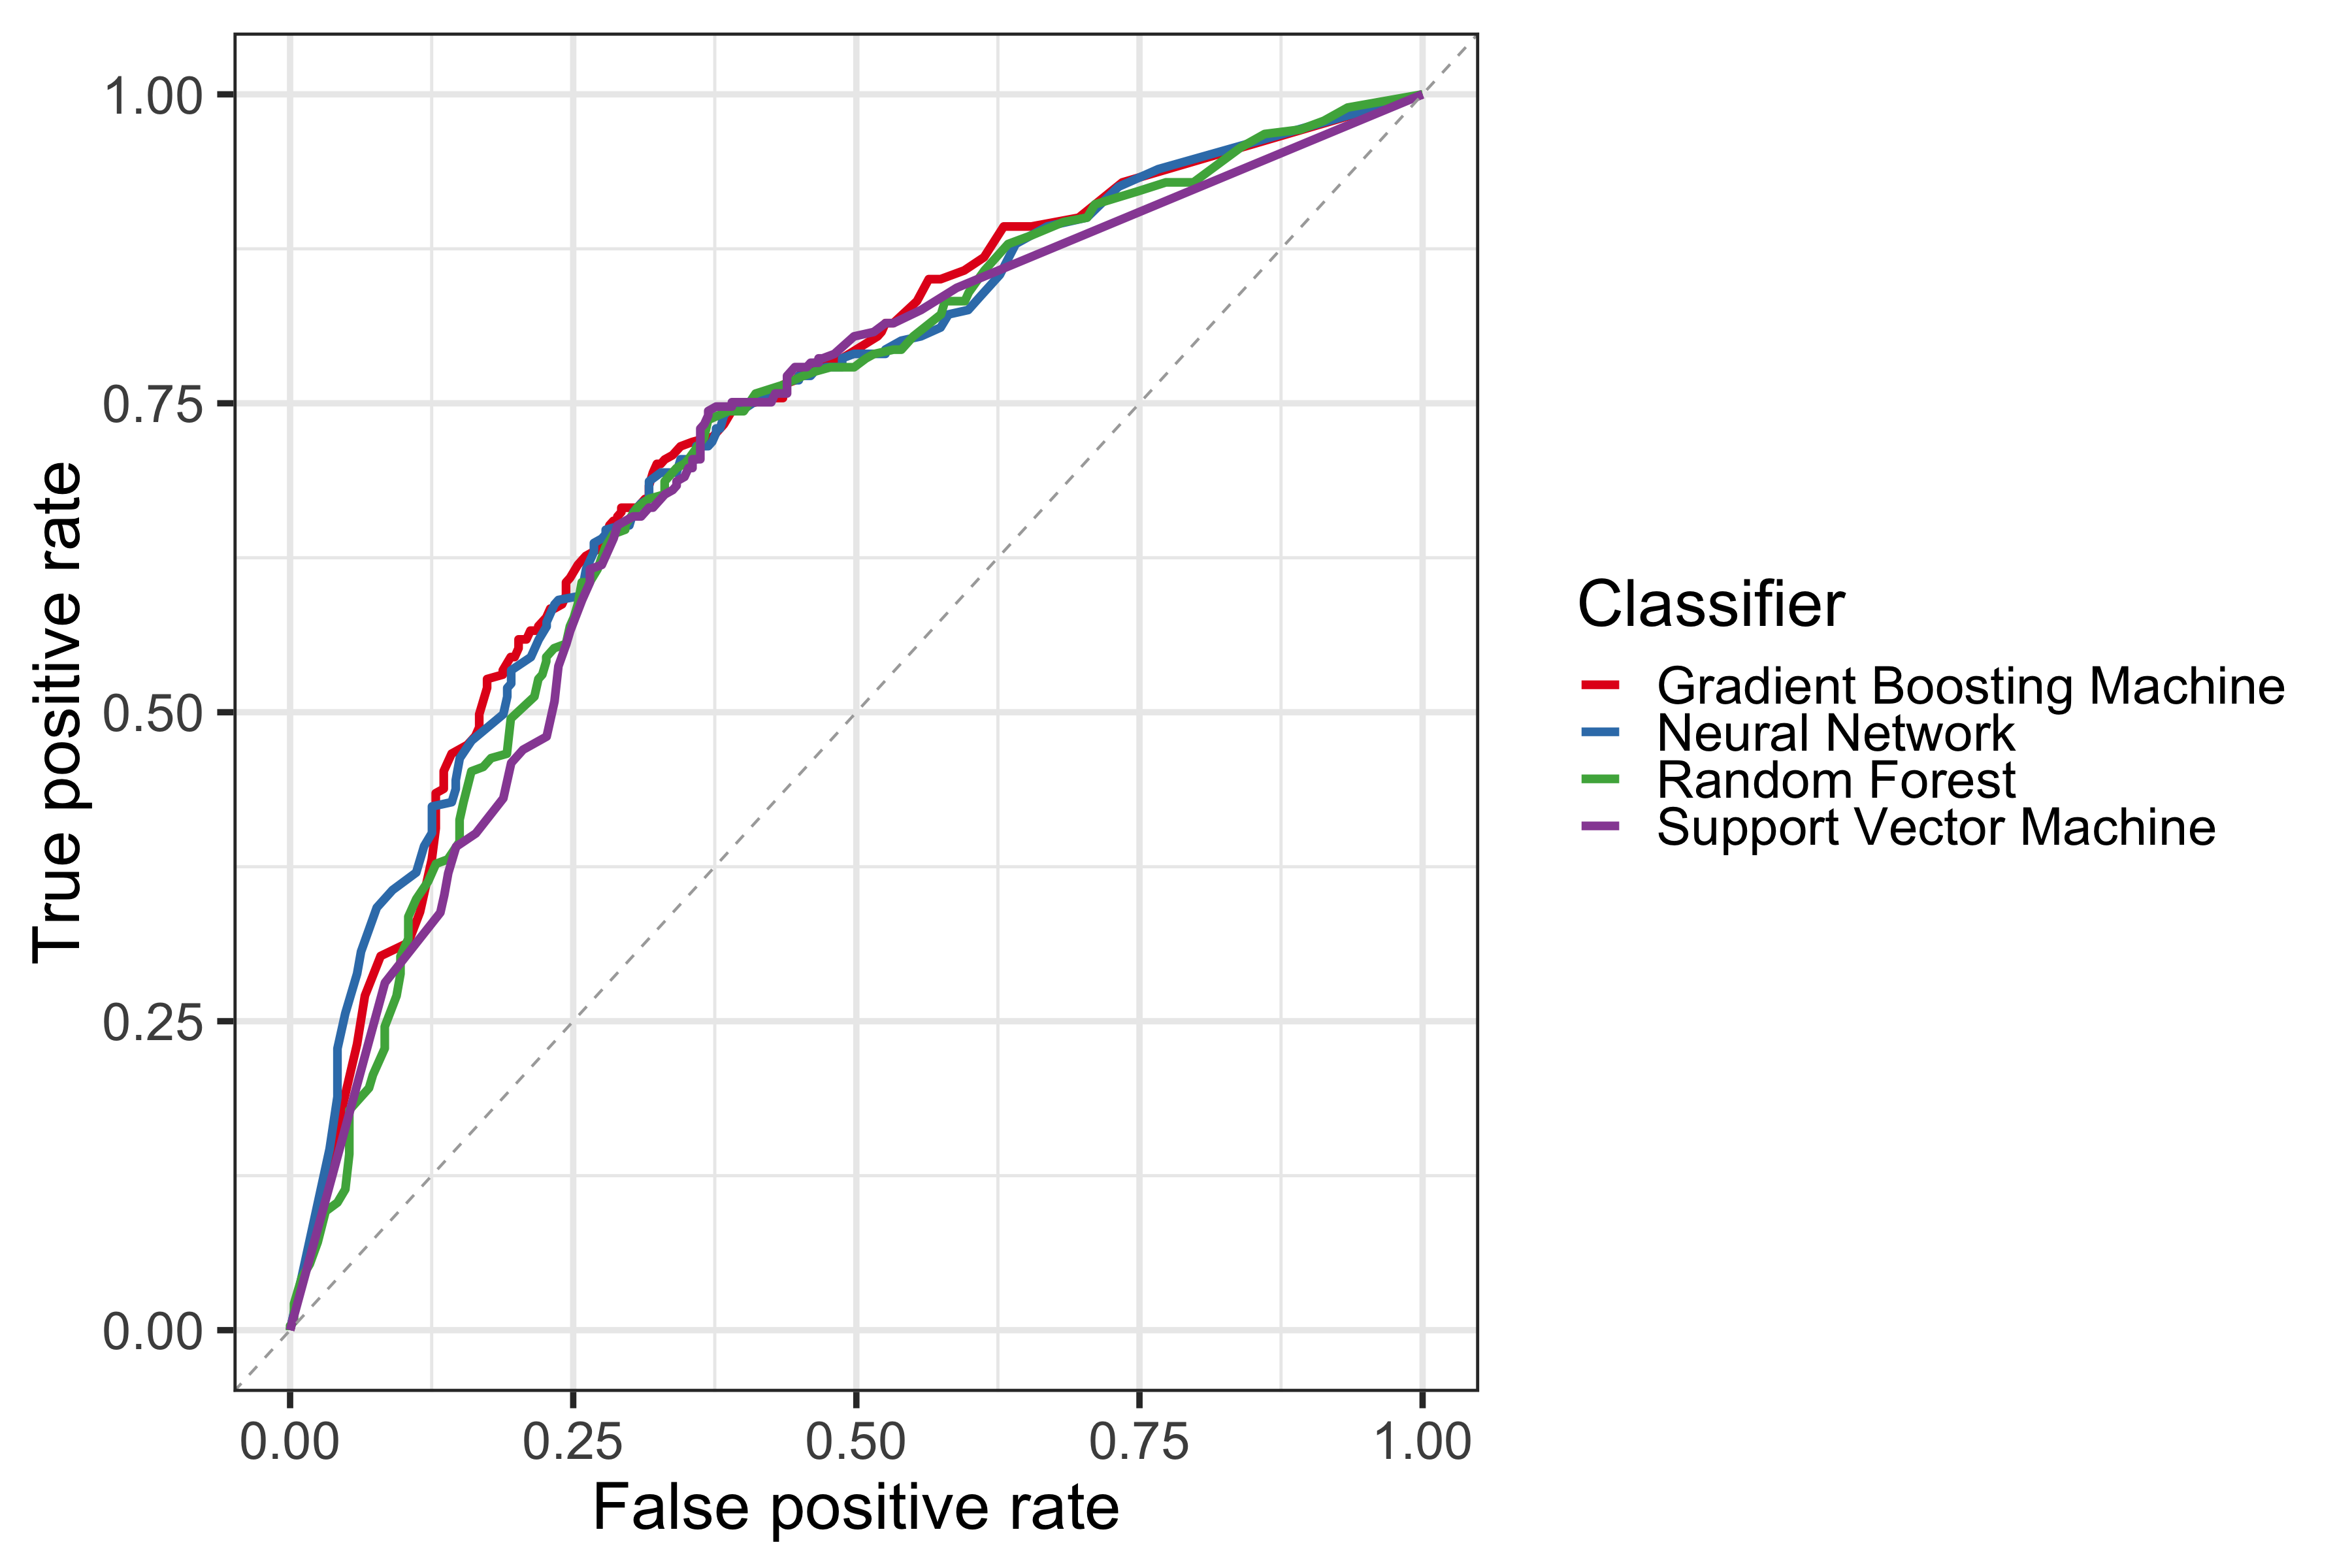
\includegraphics[width=11cm]{pics/BenchmarkROC.png}
    \caption{Estimated receiver operating characteristic (ROC) curve of trained classifiers as assessed by nested cross-validation on the training set \label{fig:OT_ROC}}
\end{figure}

\begin{figure}[H]
    \centering
    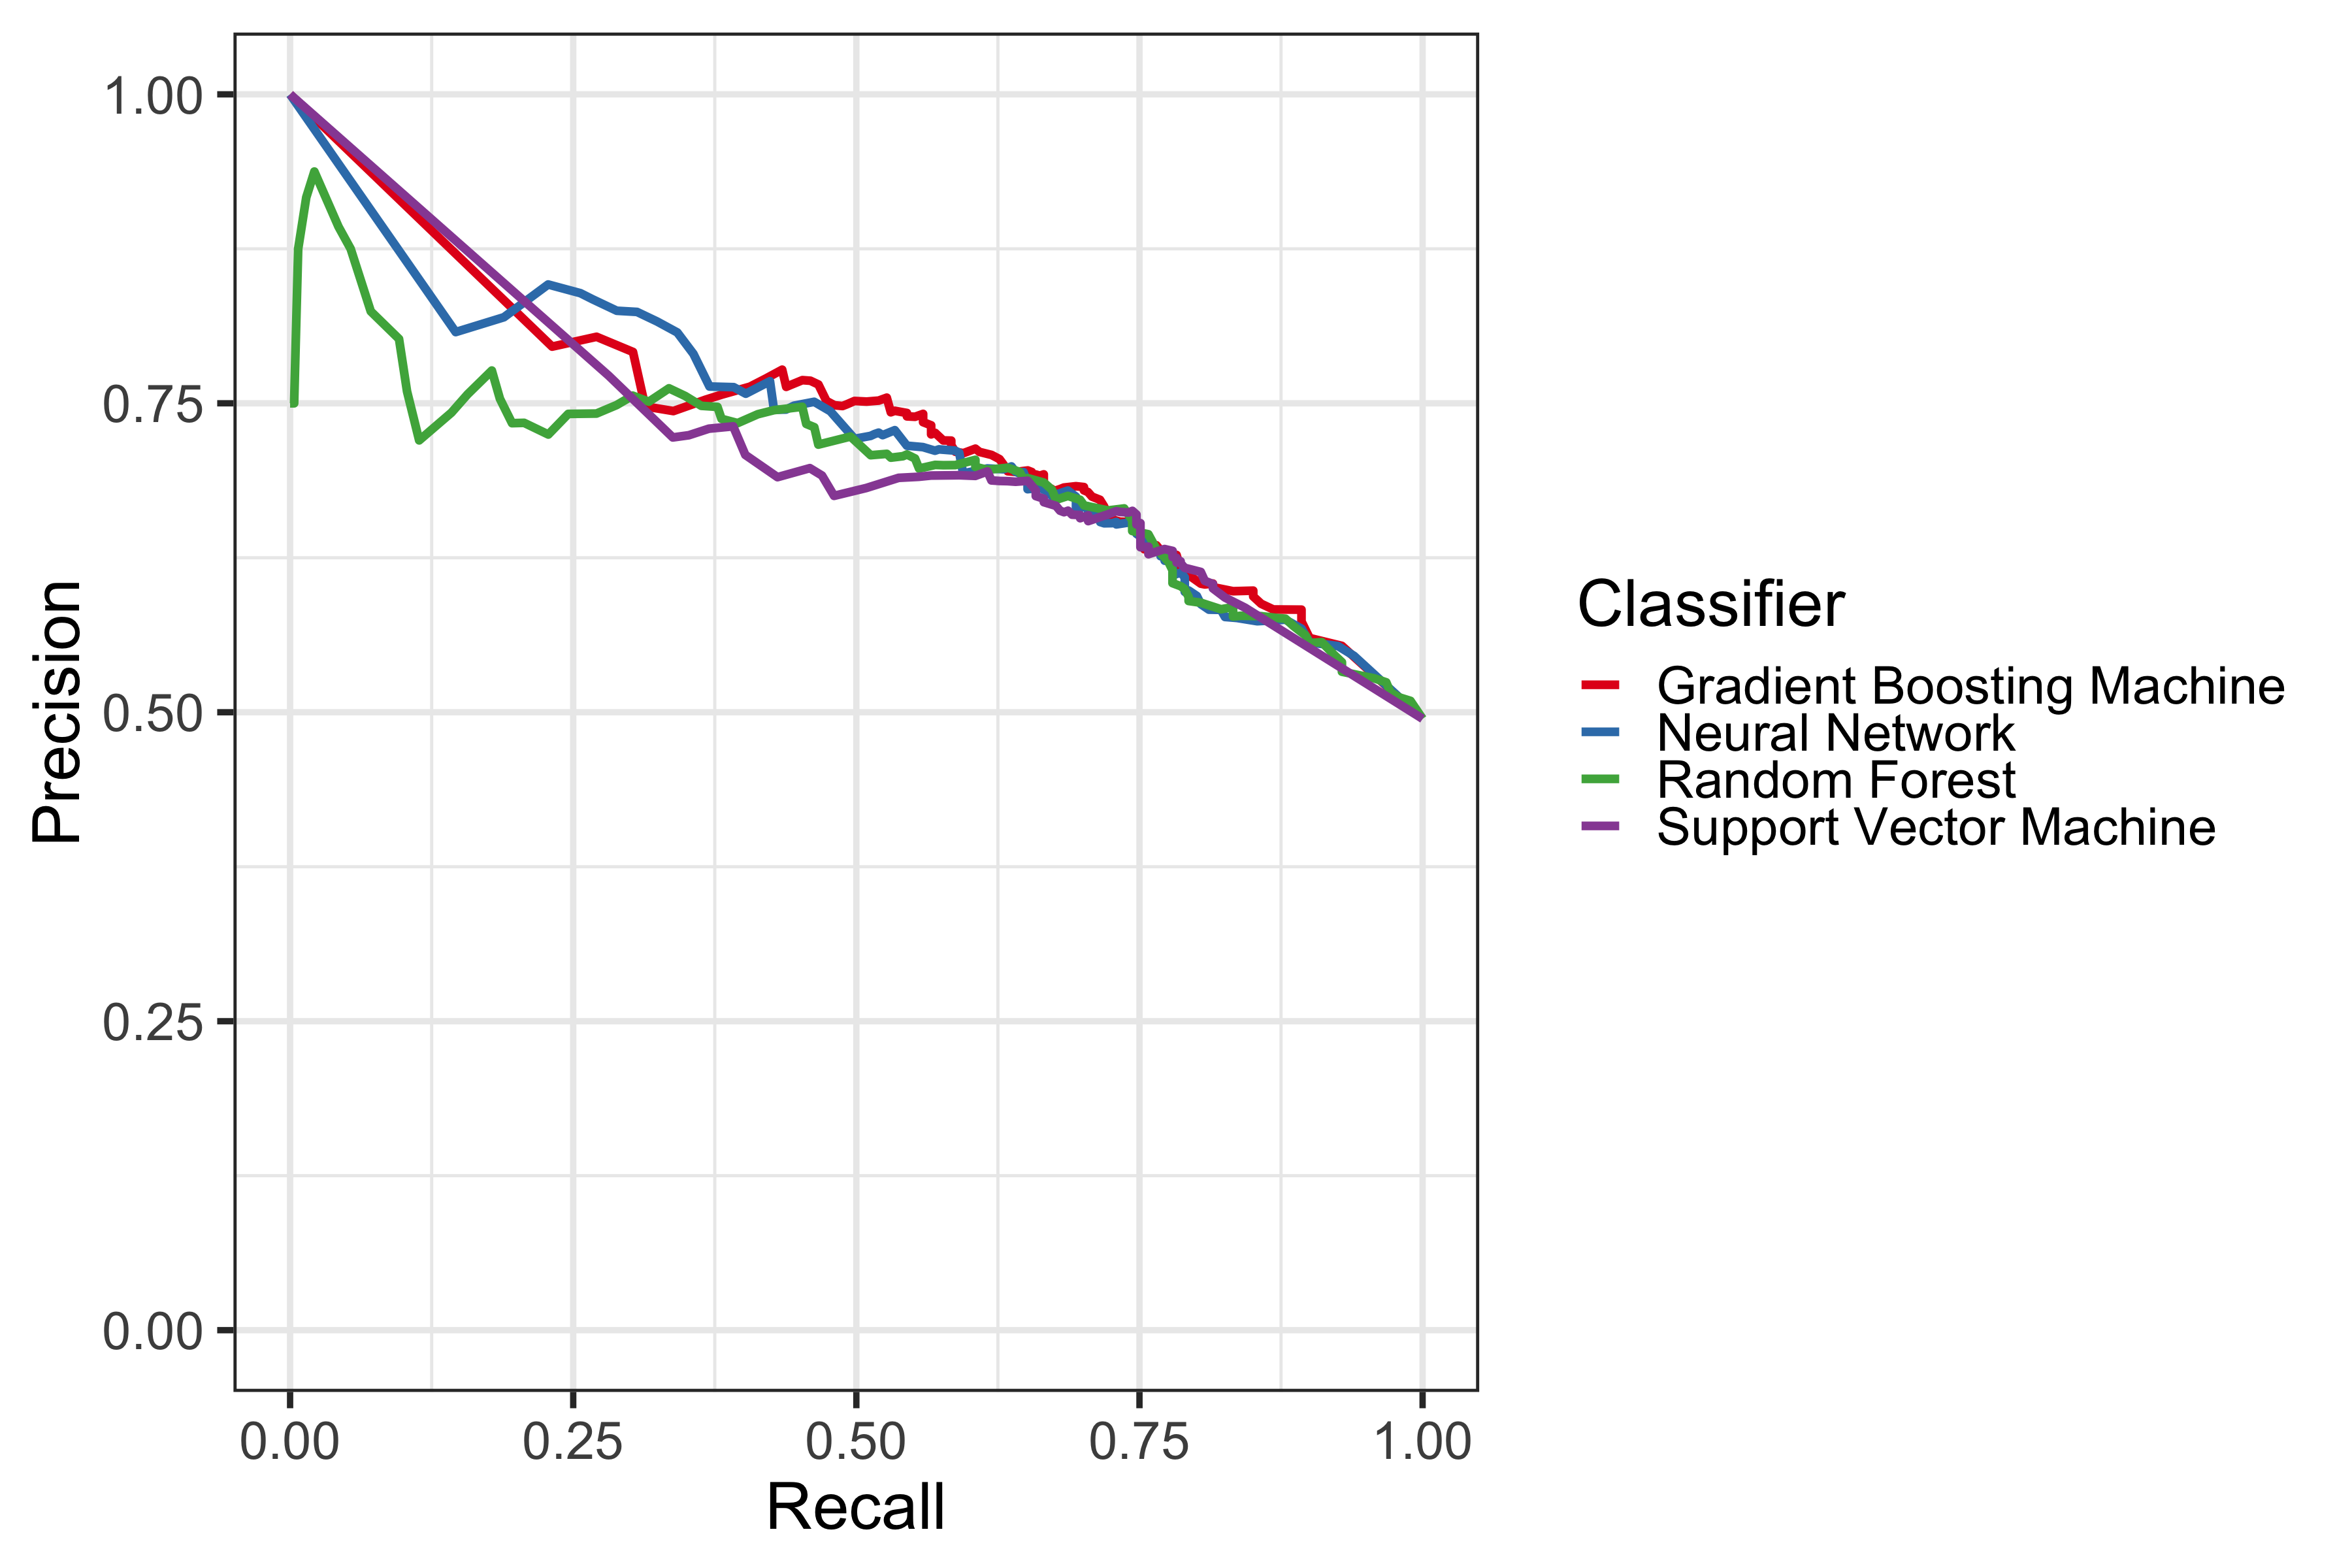
\includegraphics[width = 11cm]{pics/BenchmarkPR.png}
    \caption{Precision-–recall curves of the four trained classifiers as assessed by NCV on the \texttt{training set} \label{fig:OT_precisionRecall}}
\end{figure}

\begin{figure}[H]
    \centering
    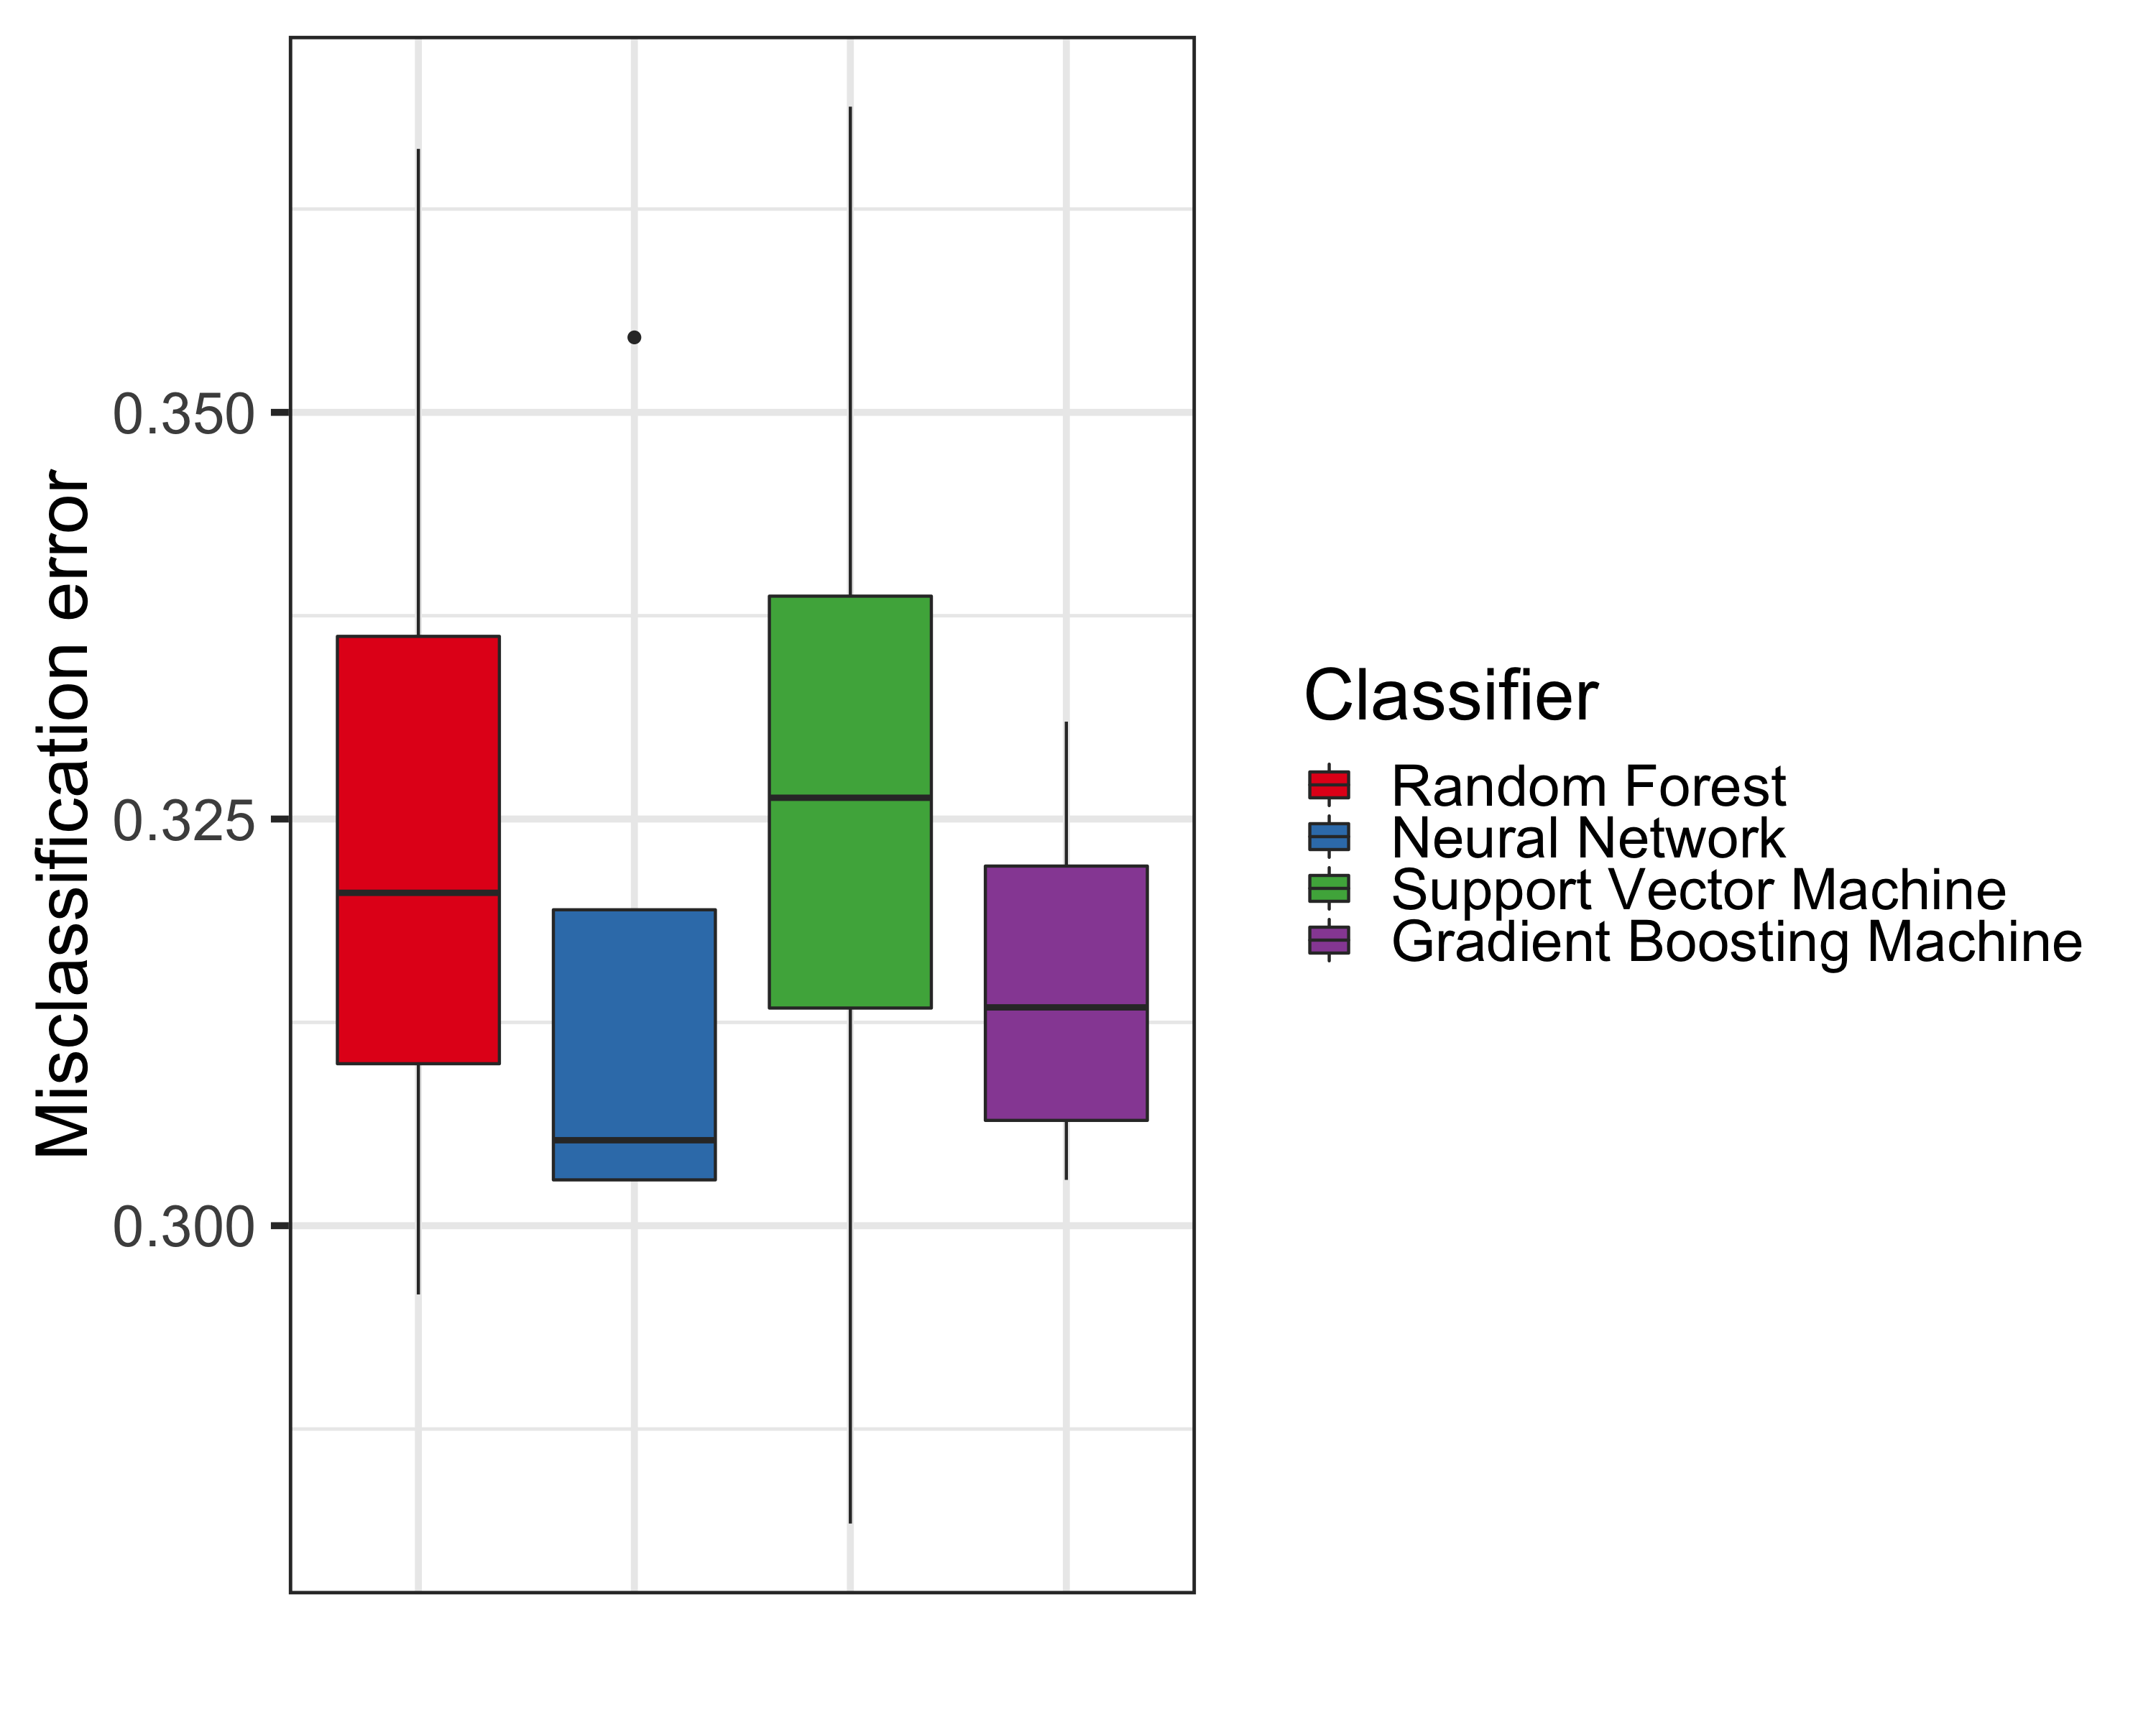
\includegraphics[width = 9cm]{pics/BenchmarkMmceBoxplots.png}
    \caption{Box plot showing the distribution of misclassification errors for the four trained classifiers, as assessed by NCV on the \texttt{training set} \label{fig:OT_MmceBoxplots}}
\end{figure}

\begin{figure}[H]
    \centering
    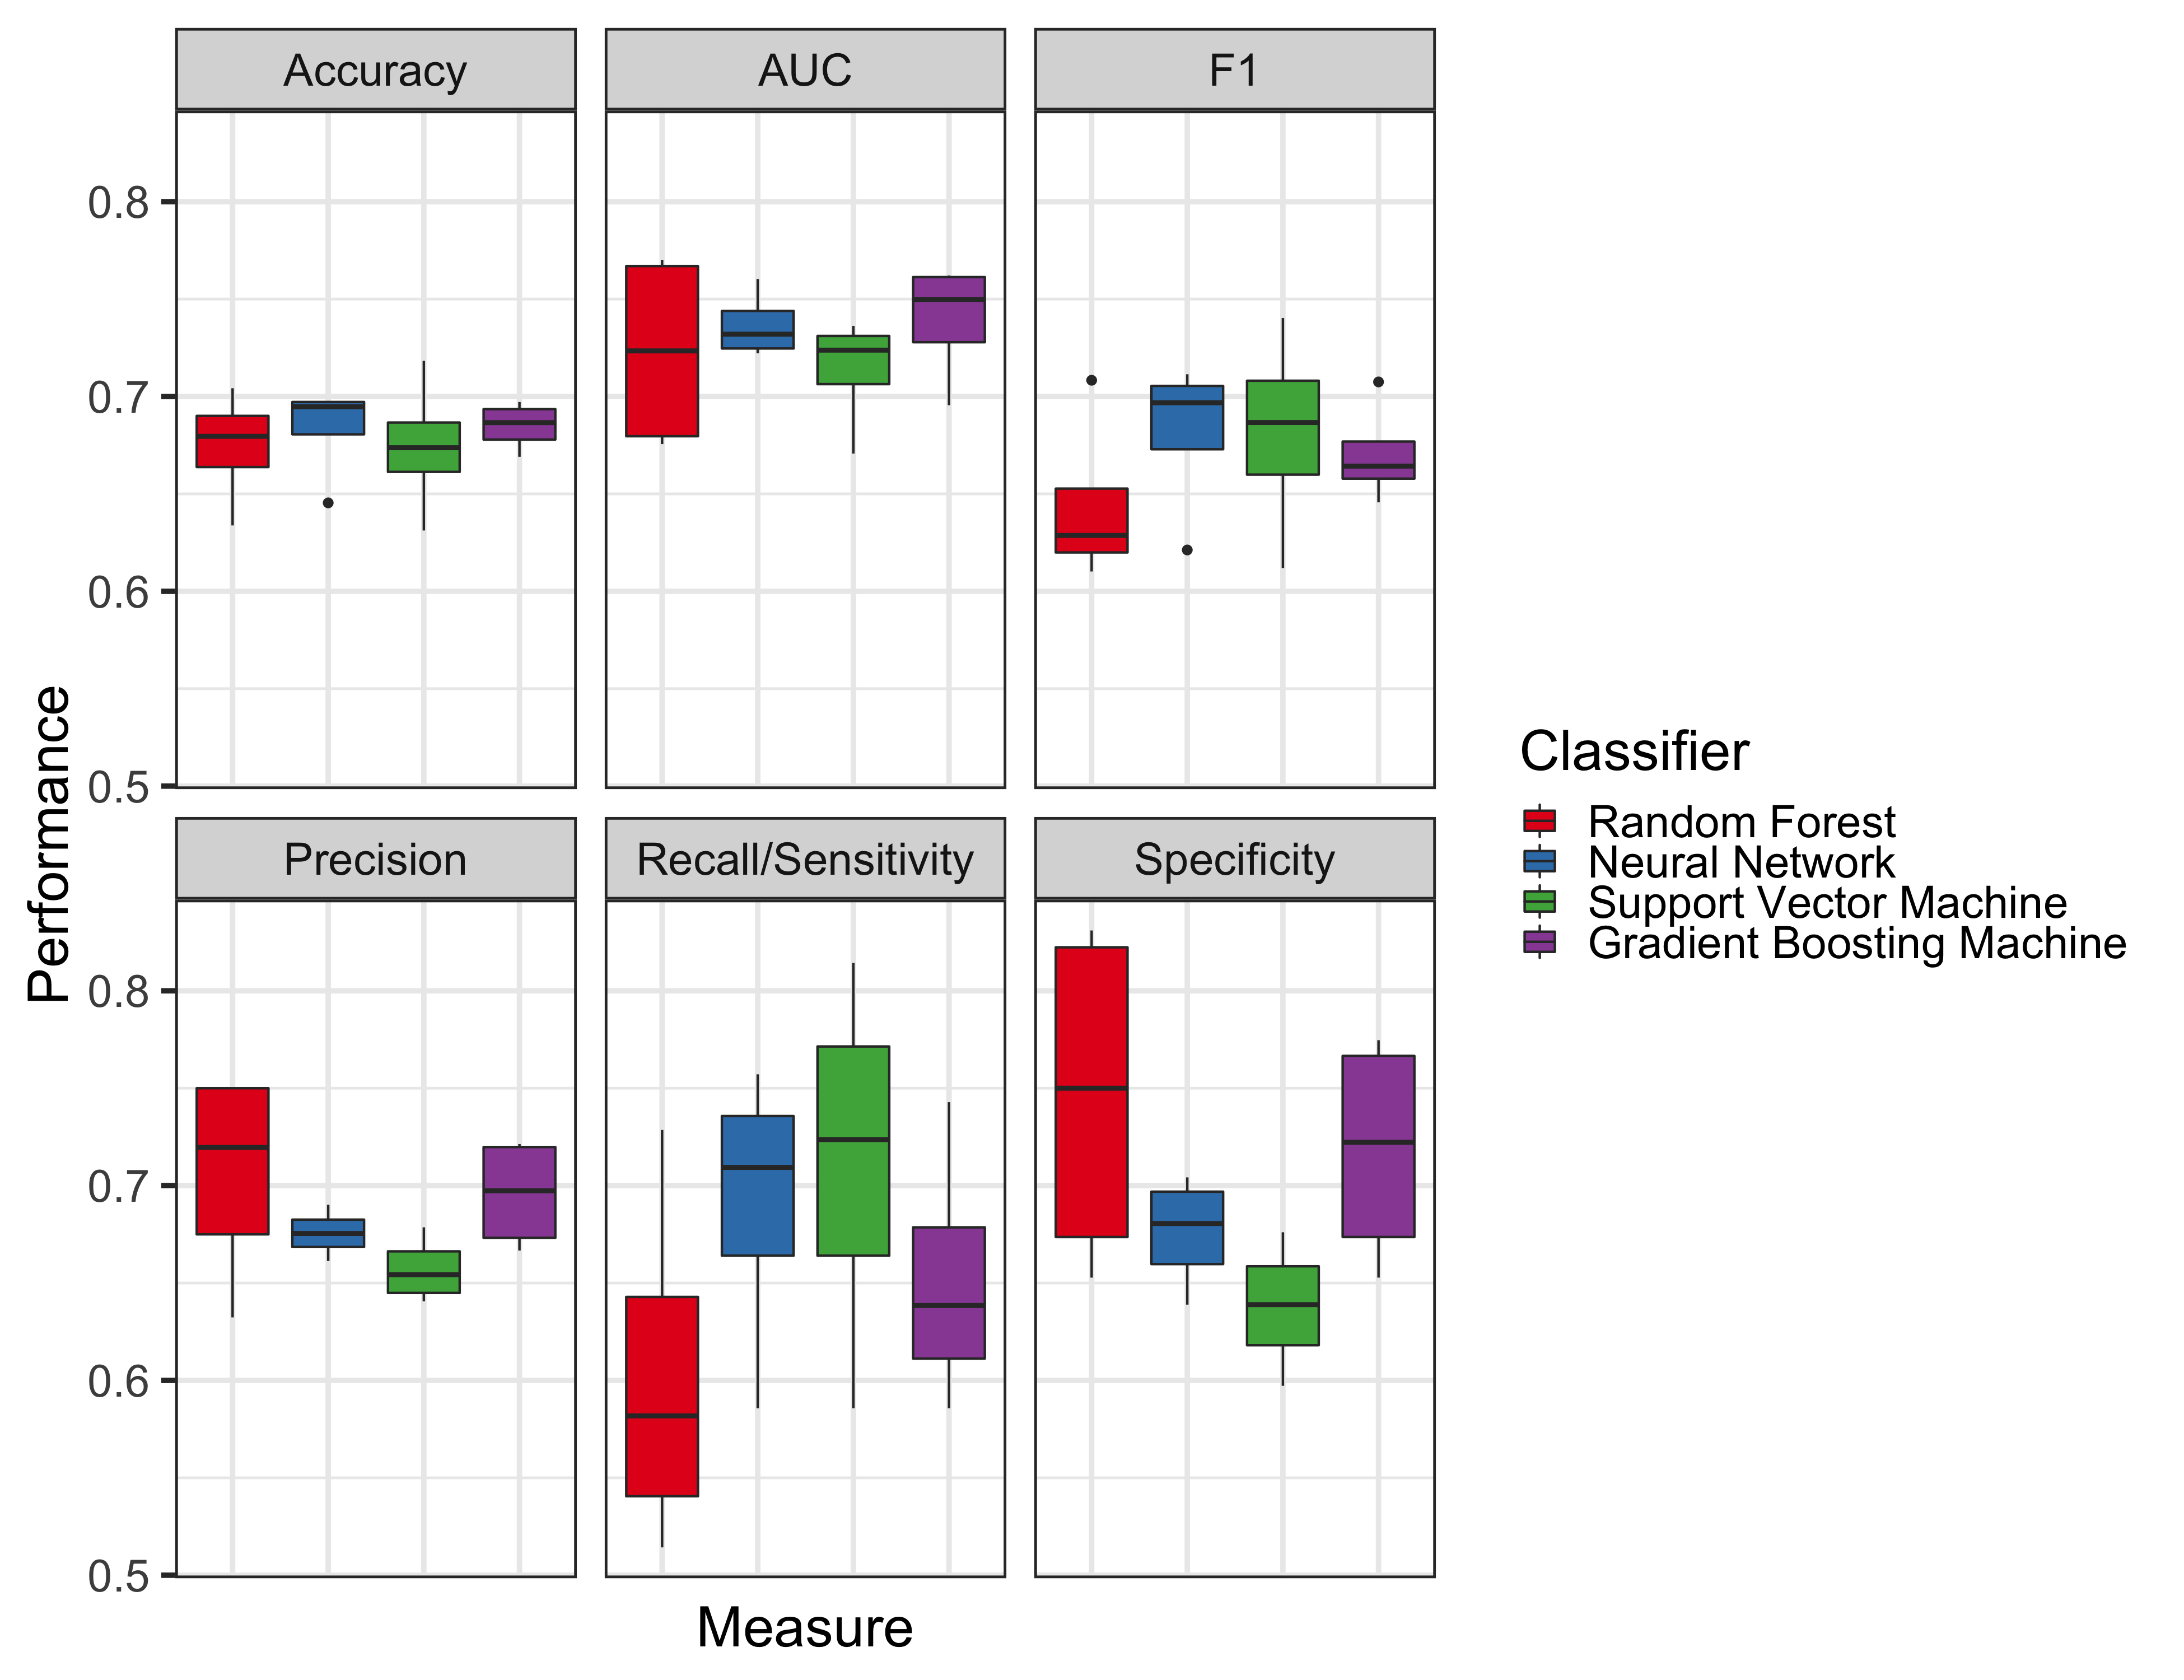
\includegraphics[width = 13cm]{pics/BenchmarkOtherBoxplots.png}
    \caption{Box plots showing distributions of the following measures for the four trained classifiers: accuracy, AUC, F1 measure, precision, recall/sensitivity and specificity, as assessed by NCV on the \texttt{training set} \label{fig:OT_OtherPlots}}
\end{figure}

Overall, all algorithms had comparable accuracy, AUC, and precision (see Figure \ref{fig:OT_OtherPlots}). These results are slightly lower than the ones reported by Ferrero et al. \cite{ferrero2017} (See my results in Table \ref{tab:David_perf_train_mean} and Ferrero's results in Table \ref{tab:OT_perf_train_mean}). 

\begin{table}[H]
\centering
\begin{tabular}{c|c|c|c|c|c|c|c}
Classifier & MMCE  & Accuracy   & AUC   & Recall/Sensitivity   & Specificity   & Precision   & F1    \\
\hline
RF & 0.326 & 0.674 & 0.723 & 0.602 & 0.746 & 0.705 & 0.644 \\
NN & 0.317 & 0.683 & 0.737 & 0.690 & 0.676 & 0.676 & 0.682 \\
SVM & 0.326 & 0.674 & 0.714 & 0.712 & 0.638 & 0.657 & 0.681 \\
GBM & 0.315 & 0.685 & 0.739 & 0.651 & 0.718 & 0.696 & 0.670
\end{tabular}
\caption{\textbf{David results}. Mean \texttt{training set} performance measures (mean misclassification error, mean accuracy, mean AUC, mean recall/sensitivity ratio, mean specificity, mean precision, mean F1 measure) for all classifiers estimated by NCV \label{tab:David_perf_train_mean}}
\end{table}

\begin{table}[H]
\centering
\begin{tabular}{c|c|c|c|c|c|c|c}
Classifier & MMCE  & Accuracy   & AUC   & Recall/Sensitivity   & Specificity   & Precision   & F1    \\
\hline
RF         & 0.302 & 0.698 & 0.761 & 0.596 & 0.802 & 0.753 & 0.665 \\
NN         & 0.303 & 0.697 & 0.758 & 0.610 & 0.785 & 0.742 & 0.670 \\
SVM        & 0.317 & 0.683 & 0.733 & 0.592 & 0.775 & 0.729 & 0.652 \\
GBM        & 0.297 & 0.703 & 0.752 & 0.637 & 0.771 & 0.738 & 0.683
\end{tabular}
\caption{\textbf{Open Targets \cite{ferrero2017}}. Mean \texttt{training set} performance measures (mean misclassification error, mean accuracy, mean AUC, mean recall/sensitivity ratio, mean specificity, mean precision, mean F1 measure) for all classifiers estimated by NCV \label{tab:OT_perf_train_mean}}
\end{table}

Finally, Ferrero et al. explored how consistent was the target predictions across all four trained binary classifiers in the \texttt{training set}. All four algorithms agreed on the classification of the majority of the observations in the \texttt{training set} for both targets (47.74\% in my results versus 66.4\% in Ferrero et al.) and non-targets (55.55\% in my results versus 75.2\% in Ferrero et al.). Venn diagrams are in Figure \ref{fig:OT_venn}.

\begin{figure}[H]
\resizebox{\textwidth}{!}{
    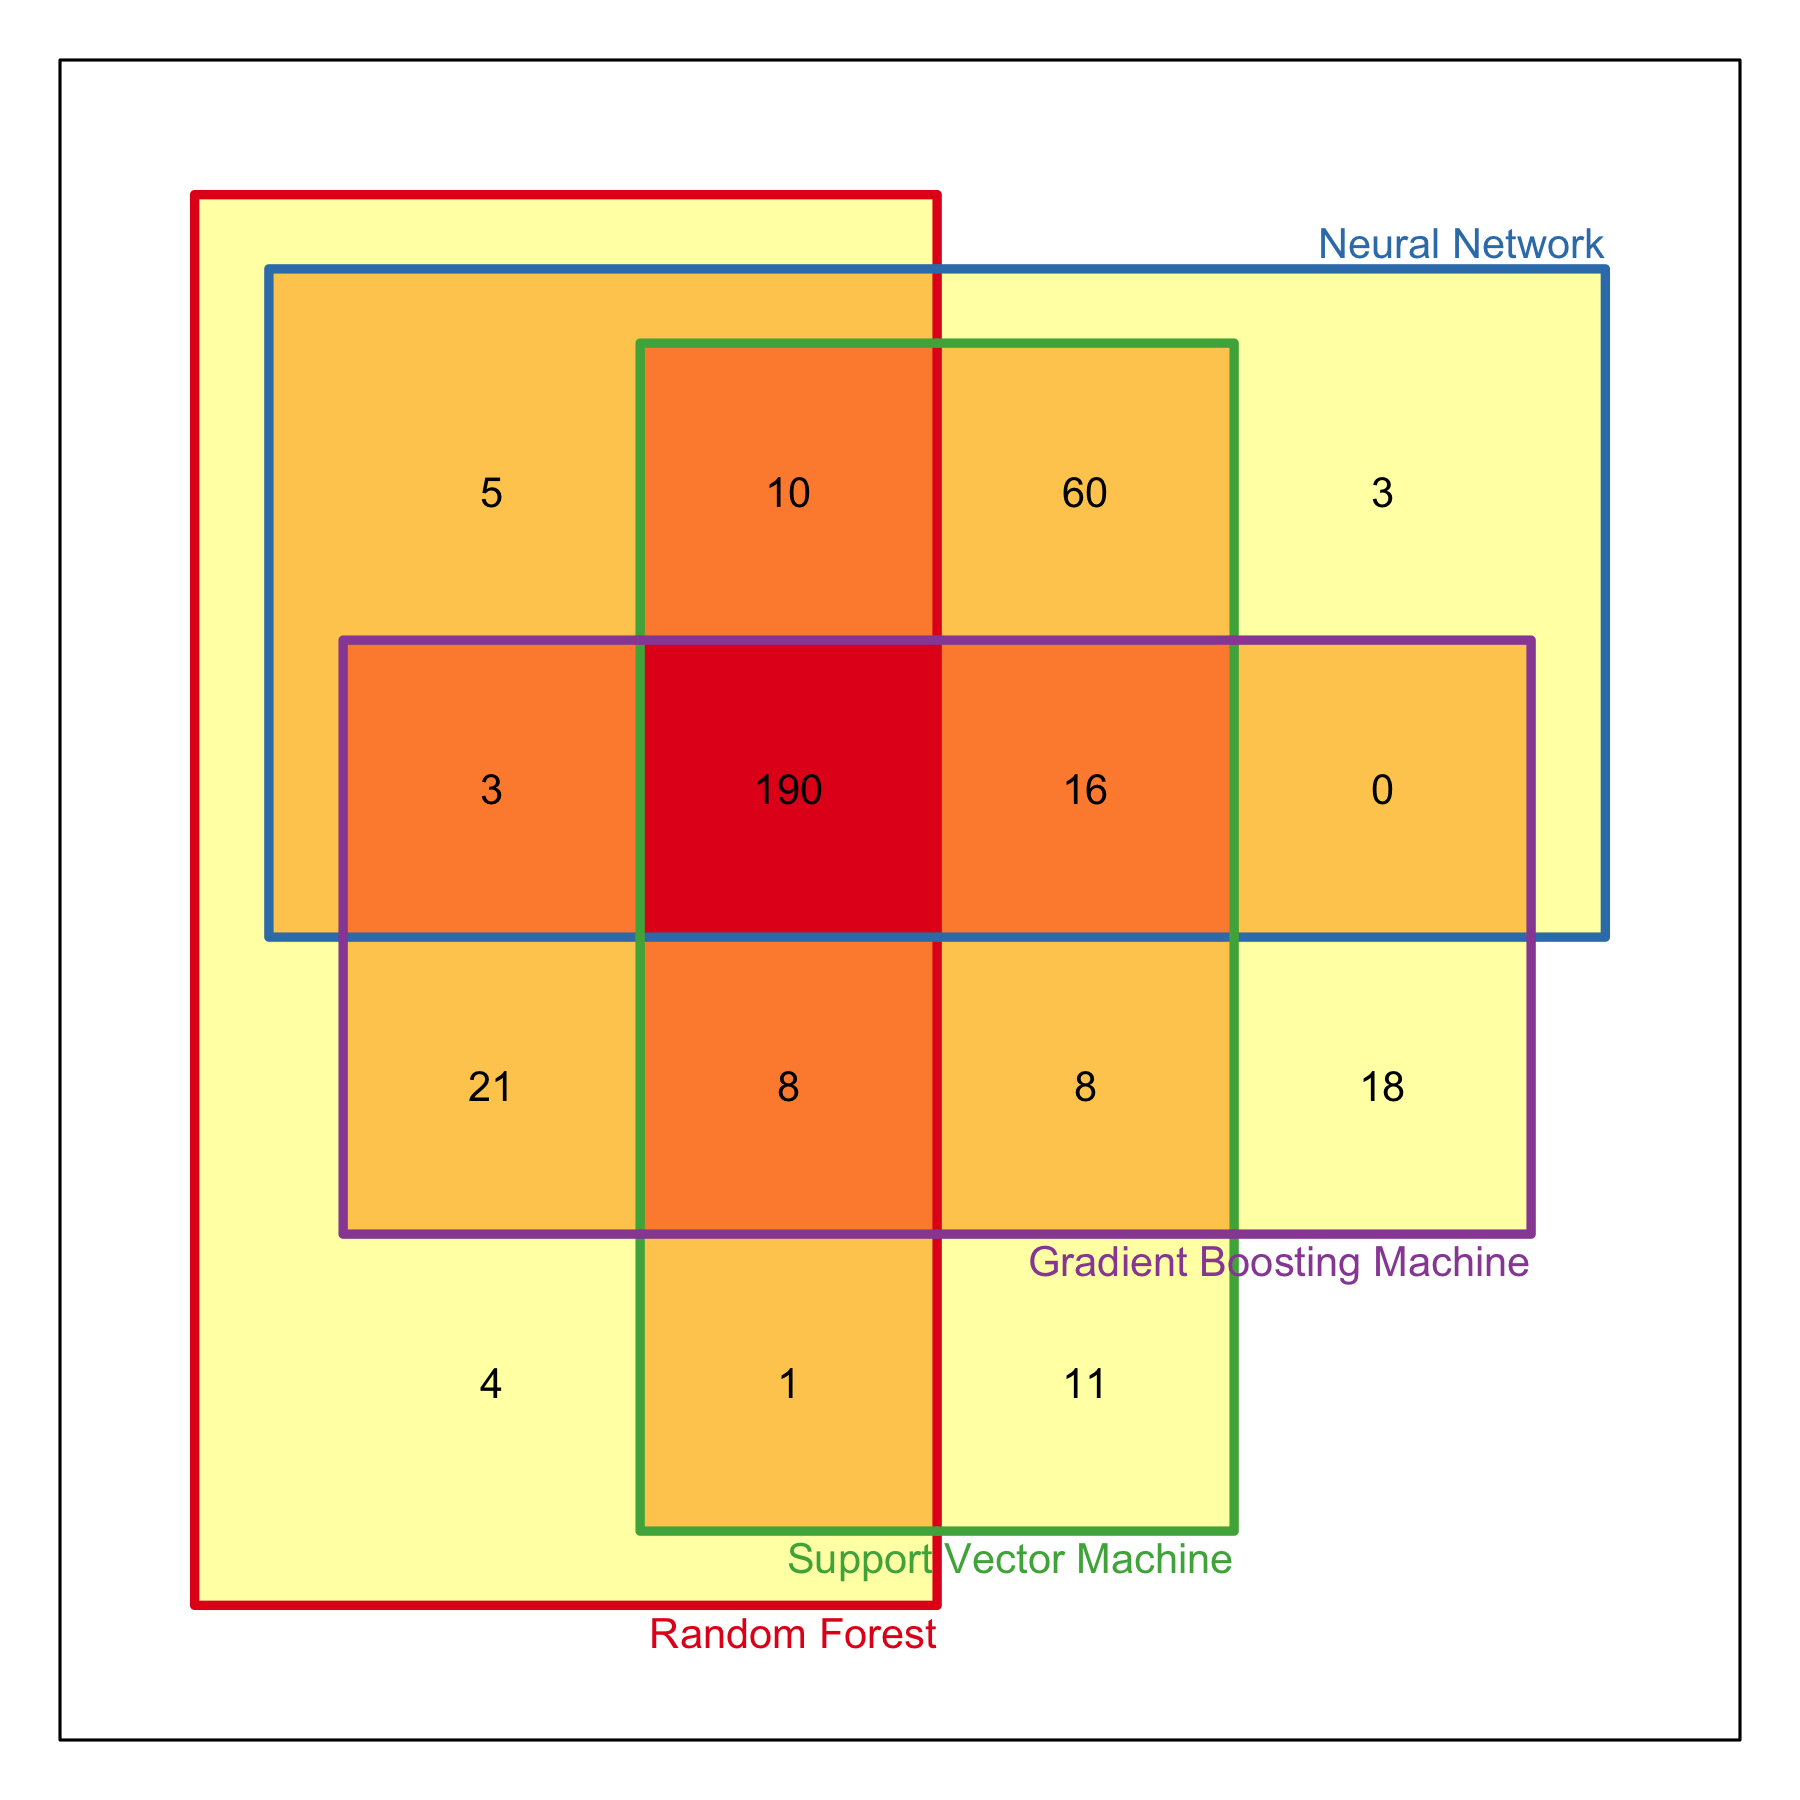
\includegraphics{pics/VennTargets.png}
    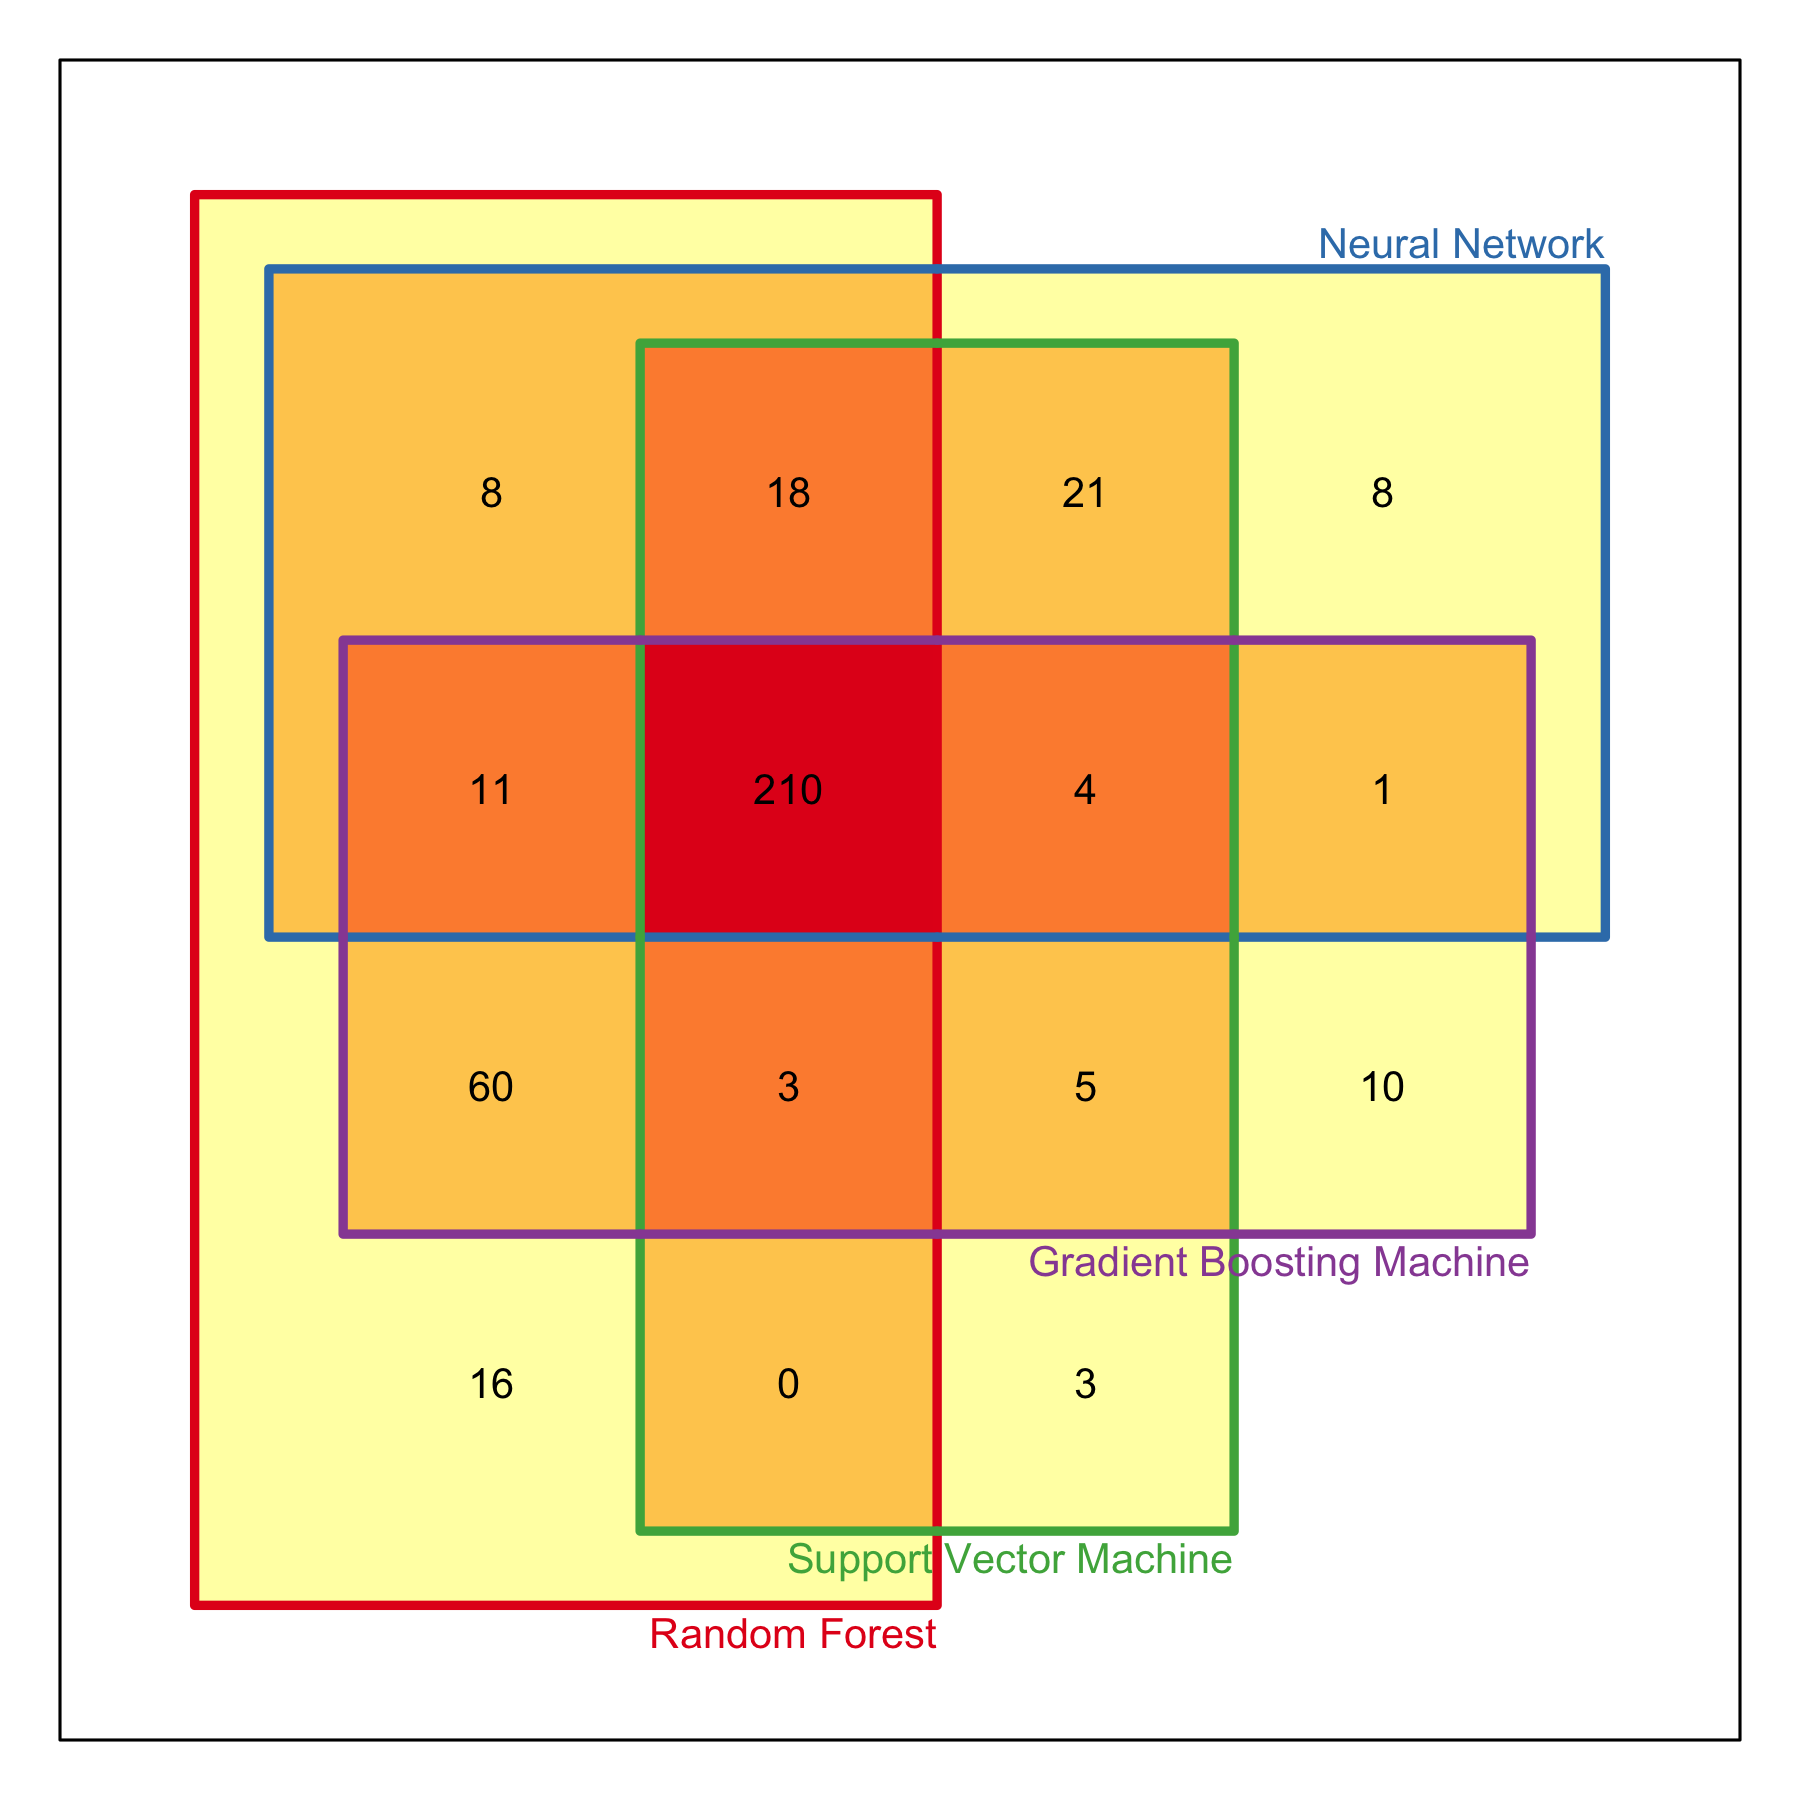
\includegraphics{pics/VennNontargets.png}}
    \caption{Overlap of predicted targets across the four trained classifiers. Venn diagrams showing the relative overlap of predicted targets (left) and predicted non-targets (right) from the \texttt{training set} for the four trained classifiers \label{fig:OT_venn}}
\end{figure}

To further ensure that they were not overfitting the models to the training data, they also evaluated the performances of the four classifiers on the \texttt{test set} (see Figure \ref{fig:ot_workflow}) that was not previously fed in the training of the binary classifiers. The performance of all four trained models was consistent with the NCV results on the \texttt{training set} in both Ferrero et al. \cite{ferrero2017} and my results (see Table \ref{tab:David_perf_train_mean}). This indicates that overfitting did not occur.

\begin{table}[H]
\centering
\begin{tabular}{c|c|c|c|c|c|c|c}
Classifier & MMCE  & Accuracy   & AUC   & Recall/Sensitivity   & Specificity   & Precision   & F1    \\
\hline
RF & 0.289 & 0.711 & 0.720 & 0.649 & 0.779 & 0.762 & 0.701 \\
NN & 0.296 & 0.704 & 0.698 & 0.730 & 0.676 & 0.711 & 0.720 \\
SVM & 0.303 & 0.697 & 0.722 & 0.743 & 0.647 & 0.696 & 0.719 \\
GBM & 0.373 & 0.627 & 0.664 & 0.622 & 0.632 & 0.648 & 0.634
\end{tabular}
\caption{\textbf{David results}. \texttt{Test set} performance measures (misclassification error, accuracy, AUC, recall/sensitivity ratio, specificity, precision, F1 measure) for all trained classifiers \label{tab:OT_perf_test}}
\end{table}

\subsubsection{TO DO}
\begin{itemize}
    \item Predicted targets in the \texttt{prediction set}
    \item Histograms for different stages or phases of development (Data from PharmaProjects)
    \item Literature text mining for validation (I do not have this data from Docstore)
\end{itemize}

An intrinsic limitation of validation methods for ML is the use of the same source of information as a label \cite{ferrero2017}. Ferrero et al. used \textbf{scientific literature} as an external source of information for the validation. Concretely, they mined co-occurrences of gene or proteins being flagged as potential therapeutic targets in titles and abstracts of published articles in MEDLINE \cite{ferrero2017}. They found 25,603 GDAs, corresponding to 4413 unique genes\cite{ferrero2017}. 590 of these 4413 genes were in common with the predicted targets by the trained NN model, a highly significant proportion as assessed by Fisher’s exact test (p = 5.05e−172, odds ratio = 5.78) \cite{ferrero2017}

\subsubsection{Limitations}
\label{subsub:limitations_openTargets}
\begin{itemize}
    \item \textbf{Labelling of the classes}: there is no pure negative nor positive class which complicates the problem of a binary classification: defining \emph{bona fide} unsuccessful targets is extremely difficult, if possible at all.
    
    Failed or abandoned projects according to Informa Pharmaprojects were ignored \cite{ferrero2017}. It is unclear the why the projects failed or were abandoned: (i) one target could be perfectly viable but it may have been withdrawn for commercial or R\&D reasons or (ii) unsuccessful targets in one area may be valuable in others.
    
    Ferrero et al. \cite{ferrero2017} assumed that the unlabelled, negative set contained both future positive targets, not being actively pursued as therapeutics, and negative targets for any reason. From an algorithmic perspective, they simply treated the unlabelled data as the negative set, allowing them to use supervised learning methods within a semi-supervised setting according to \cite{elkanUnlabelled2015}. Nonetheless, for this reason, (i) the number of true positives is going to be underestimated or, in other words, (ii) the false positive rate is overestimated, leading to worse precision and sensitivity/recall estimates \cite{ferrero2017}.
    
    Additionally, some drugs in early stages of drug development were defined as \emph{positive} successful targets but they may fail in latter stages.
    
    \item In terms of performance, the NN model was the best with a 71\% accuracy even though no classifier significantly outperformed the others. Nevertheless, this is not a great performance. Can I do better including more data types or using different ML algorithms?
    
    \item  Inclusion of functional (Gene Ontology, pathways), structural (protein domains) or interaction data (protein–-protein interactions) is likely to have a large impact on the ability to successfully predict therapeutic targets as it has been already demonstrated \cite{ferrero2017}. Ferrero et al. did not considered these data types.
    
    \item Their model correctly classified later stage drug targets more easily than earlier stages targets.  Therapeutic targets more advanced in the drug discovery pipeline show clearer differences and thus appear more straightforward to discriminate \cite{ferrero2017}.
    
    \item Their predictions were individual targets, and not target–-indication or target--disease pairs: they predicted potential therapeutic targets, regardless of the intended indication.
    
    \item Ferrero et al. did not make any claim regarding the druggability of these targets. Open Targets answers questions focused on GDAs but is unable to report focused aspects about the bioactivity profiles of small molecules on those targets \cite{brown2018}
    
    \item Ferrero et al. removed the feature \texttt{literature} since it it was likely to be heavily biased towards well known, validated target–indication pairs and, in addition, they used it to validate their approach. What about \texttt{animal\_model}?
    
    \item Why \texttt{animal\_model} is a good feature for predicting (like they say in the title!) \textbf{novel} therapeutics? Is not just a mere reflection of how much effort has been put on a given GDA? How much money has already been invested in deciphering a GDA? How much time has been spent or even lost in a GDA? How novel targets are going to have high scores in \texttt{animal\_models}? Ferrero et al. \cite{ferrero2017} reported that the algorithm was able to predict much better genes that had pharmaceutics in the market. Is not that obvious? Are not genes with human orthologs in animals been studied in clinical phases before being launched to the market?
    
    Stoeger and colleagues \cite{stoeger2018} demonstrated that the impact of research on model organisms particularly influenced research in human genes. Furthermore, Homologous genes of unstudied human genes are likewise unstudied in model organisms.
    
    Because if there is a high score in the \texttt{animal\_model} feature, it can mean to things: (i) the GDA is already well defined, well studied before doing the animal model and there is a target for it or (ii) the GDA has been a failure and there is no target yet.
\end{itemize}

Finally, Ferrero et al. \cite{ferrero2017} reported that they did not neglected inference. They report that their decision tree gains some insights into the characteristics that makes good therapeutic targets \cite{ferrero2017}. But, the main feature in the decision tree is \texttt{animal\_model}. How do they infer this? Where is the causality? How making an experiment in an animal converts a target in a good target? It just turns out that no one, surprisingly, is going to waste resources in experimenting with animals without enough evidences. What if we made animal experiments in all human ortholog genes? Would all these genes be good targets? Their research is just based on prediction! There is no causal inference anywhere.

Focusing on the publications reporting the discovery of new human genes, we found an overrepresentation of publications that cite studies of nonhuman genes (Figs 2D and S6A). Inspecting the organisms of these genes, we observed two classes of organisms. The first class preferentially co-occurred together with human genes and consisted of Mus musculus, Rattus norvegicus, Bos taurus, and Gallus gallus (37%, 9.1%, 2.6%, 2.5% of all citations, respectively). The second class preferentially occurred in publications without human genes and consisted of Drosophila melanogaster, Saccharomyces cerevisiae, Escherichia coli, Xenopus laevis, Caenorhabditis elegans, and Schizosaccharomyces pombe (22%, 10%, 4.0%, 2.5%, 1.6%, 1.5% of all citations, respectively) (S6B Fig). Assuming that citations are one proxy of scientific impact, this finding suggests that initial reports on human genes have been particularly influenced by research in model organisms and that multiple model organisms have contributed complementary roles in the discovery of human genes.

With these insights, we dramatically increased the prediction accuracy of the year of initial report of a human gene by including the years of the initial reports on homologous genes of model organisms (Fig 2E, from Spearman: 0.48 to 0.71). Moreover, the years of the initial reports on homologous genes improved prediction accuracy of the number of publications to a greater extent than the year of the initial report on the human genes themselves (S7A Fig, Spearman: 0.81).

Consistent with the picture emerging from these analyses, the homologous genes of unstudied human genes are likewise unstudied in model organisms (S6 Table), and including the number of publications on homologous genes yielded almost perfect predictions of the number of publications for individual human genes (Fig 2F, Spearman: 0.87), while human-specific genes without homologous genes remain significantly less studied (S7B Fig, Mann–Whitney U test: p-value < 10−32). Taken together, these findings demonstrate the impact of research on model organisms on the knowledge acquired on human biology—a hypothesis that had been proposed but not demonstrated previously [32].

% PHAROS
\newpage
\subsection{PHAROS}
\label{subsec:pharos}



 
The \href{https://druggablegenome.net/}{Illuminating the Druggable Genome} was a programme initiated by the National Institutes of Health (NIH) in 2014 and today is a worldwide collaboration between the University of New Mexico, Icahn School of Medicine, Mount Sinai, EMBL-EBI, the Novo Nordisk Foundation Center for Protein Research (University of Copenhagen), and the University of Miami \cite{pharos2016}.  Created in 2014, IDG was initially motivated to shed light to 1700 targets from four privileged drug target families \cite{santos2016}: G-Protein Coupled Receptors (GPCRs), kinases, ion channels, and nuclear receptors \cite{pharos2016}. Nevertheless, IDG is moving beyond those 4 families and now considers all 20k human coding genes \cite{pharos2016} based on phylogenecity, function, target development level, disease association, tissue expression, chemical ligand and substrate characteristics, and target-family specific characteristics. They developed the \href{http://drugtargetontology.org}{Drug Target Ontology (DTO)} \cite{lin2017}, also available on \href{http://github.com/DrugTargetOntology/DTO}{GitHub} and the \href{http://bioportal.bioontology.org/ontologies/DTO}{NCBO Bioportal}.

\noindent IDG has two distinct resources:

\begin{itemize}
    \item \href{http://juniper.health.unm.edu/tcrd/}{Target Central Resource Database (TCRD)} is the central resource behind the Illuminating the Druggable Genome Knowledge Management Center (IDG-KMC)
    
    \item \href{https://pharos.nih.gov/idg/index}{PHAROS}, as the library of Alexandria ($\phi \alpha \rho o \zeta$), is the user interface that presents TCRD information
    
\end{itemize}

\subsubsection{Data}
\begin{itemize}

    \item TCRD can be downloaded \href{http://juniper.health.unm.edu/tcrd/download/}{here}
    
    \item Information about its content can be found \href{http://habanero.health.unm.edu/tcrd/old/content.html}{here}
    
    \item A list of the datasources used can be found \href{http://targetcentral.ws/Pharos}{here}
    
\end{itemize}

Among PHAROS resources is \href{http://amp.pharm.mssm.edu/Harmonizome/about}{Harmonizome}, that aims to integrate a wide collection of public, disjoint datasets from multiple, internationally recognised datasets (n=114 in October 2018) from 66 different databases that gather information about genomics, epigenetics, transcriptomics, metabolomics, cell lines, diseases, physical interactions, drugs, and curated biomedical literature about mammalian cells \cite{harmonizome2016}. Actualised statistics of Harmonizome can be found \href{http://amp.pharm.mssm.edu/Harmonizome/about}{elsewhere}.

\textbf{Problem}: Harmonizome does not contain the raw values, just values in the set ${1,-1}$. This is a big problem. What about all the information contained in p-values? GDAs with p-values are just ones or zeroes in Harmonizome.

\subsubsection{Scores}

\begin{itemize}
    \item \texttt{novelity\_score} as measure of extent to which the published literature refers to the target. What is the formula?
    \item \texttt{pubmed\_score} described \href{https://pharos.nih.gov/idg/pmscore}{elsewhere}
    \item \texttt{data\_availability\_score} as an indication of the current information coverage at \href{http://amp.pharm.mssm.edu/Harmonizome/about}{Harmonizome}
\end{itemize}

It is important to realize that target ranking based on individual parameters is only a first step in target prioritization. While there are examples of target prioritization using individual parameters such as GO or DO terms (21), in general, target prioritization is heavily contextual, where the context could be a disease state or a biological process.

It is possible to make comparisons between targets: \url{https://pharos.nih.gov/idg/targets/compare?q=Q05586,Q9UBN1}

\subsubsection{Limitations}
\begin{itemize}
    \item Loss of information because of the binary nature of the files: e.g. the uncertainty score of the p-value is reduced to a mere binary variable with information related to "was this gene significant?" according to an arbitrary threshold.
    
    \item 
\end{itemize}



\newpage

% Target datasources
\section{Target data sources}
What is the degree of overlap between different target databases (see Table \ref{tab:target_db_stats})?

\begin{table}[H]
    \centering
    \begin{tabular}{c|c|c|c}
         Data source & Publication & Human Ensembl & Not mapped \\
         \hline
         
         \href{https://goo.gl/VD1dTm}{TTD} &
         \cite{ttd2018} & 2415 & \href{https://goo.gl/pvWxHf}{Link}
         \\
         
         \href{https://goo.gl/Lrsyde}{DrugBank} &
         \cite{drugbank2008} & 2760 & \href{https://goo.gl/cYYa3F}{Link} \\
         
         \href{https://goo.gl/BY8yw8}{STITCH} &
         \cite{stitch42014} & &
         \\
         
         \href{https://goo.gl/mXCn7a}{PharmaGKB} &
         \cite{pharmaGSK2012} & &
         \\
         
         \href{https://goo.gl/uUPmwo}{SuperTarget} & \cite{superTarget2012} & &
         
    \end{tabular}
    \caption{Caption \label{tab:target_db_stats}}
\end{table}

Attention should be paid to these databases and GDAs. For example, \texttt{VariantLocation-Disease} from PharmaGKB refer to variants that have ``Disease'' anotation tags. These associations can be misleading because they are not necessarily direct GDAs: the annotation for rs5275 in PTGS2:

\begin{center}
    \emph{Genotype AA is associated with increased progression-free survival and overall survival when treated with capecitabine and oxaliplatin in people with Colorectal Neoplasms as compared to genotypes GG + AG}.
\end{center}

rs5275 will be listed in the relationships file as “associated” with “Colorectal Neoplasms”, but the SNP is associated with the treatment outcome for Capecitabine and Oxaliplatin in case patients.

The extracted genes from PharmaGKB: filter GENES, filter CHEMICALS, detect unique GENES.

 
 
\newpage

% Ideas project
\section{Ideas for the project}
\subsection{What makes a good target?}

An important note is to make a clear distinction between prediction and inference, correlation and causality: while \textbf{prediction} attempts to answer the question ``which are good targets?'', \textbf{inference} answers ``what makes a good target?''.

\begin{center}
\emph{``The best way to discover a new drug is to start with an old one''}
\end{center}
\rightline{--- Sir James Whyte Black OM FRS FRSE FRCP}
\medskip

Despite the efforts of several databases to provide an exhaustive data collection on drug--targets (see Table \ref{tab:target_db_stats}, it is still a challenge to retrieve a consistent and comprehensive view of the targets of approved drugs (both small molecules and biologics) with their associated molecular efficacy targets (human and pathogen) organised by therapeutical use \cite{santos2016}. 

In the setting of a full drug discovery project, the route to validation and clinical testing can essentially be reduced to a series of questions according to \cite{brown2018}. I will collect them all in the following list:
\begin{itemize}
    \item What is the target role in the disease?
    \item In which organ it acts? Where the target is expressed? Extracellular membrane will be ideal
    
    \item Which are the risks that the modulation of one target could bring as the clinical programme advances?
    
    \item Does the target appear in a disease--relevant pathway?
    
    \item Is there supporting evidence for the hypothesis from pharmacology?
    
    \item Will animal models information translate to humans? Are there human orthologs? See this \href{https://www.youtube.com/watch?v=BK04TZbO-HY}{seminar} from Dr Melissa Haendel
    
    \item Is there evidence of causation, or ability to stratify patients?
    
    \item What is the current therapy or standard care in the disease? Is there already an effective treatment, an unmet clinical need? Is it worth developing new drugs \cite{freudenberg2018, finan2017}? 
    
    \item What is the disease prevalence \cite{freudenberg2018}? What is the specificity of the target for a single disease? Is the target pleiotropic, involved in several diseases? Is the target the core of a complex regulation pathway?
    
    \item What is the competitive landscape?
    \item How strong are all the evidences?
    \item How drug effects on targets are propagated though their corresponding pathways?
    \item 
    \textbf{Why every attempt \cite{brown2018,DISEASES2015,DisGeNET2015,ctd2017} considers the GDAs as individual, isolated associations and not part of a pathway, an ontology, a signal cascade with interconnected nodes in a network?}
     If \texttt{gene1} is associated to \texttt{disease1} and \texttt{gene2} is associated to \texttt{gene1}, why just considering the pair \texttt{gene1-disease1} and not a transmission of the triple association \texttt{disease1-gene1-gene 2}? Open Targets has already done something similar by combining GPCR and endogenous ligand disease association evidences \cite{freudenberg2018} based on the publication \cite{southan2016}. For example, genetic evidence for a disease association with an endogenous ligand may exist but the corresponding GPCR may turn out to be the better drug target due to druggability \cite{freudenberg2018}.
    
    \item What is the druggability of the target \cite{freudenberg2018, finan2017}? Unanswered by Open Targets

\end{itemize}

\subsection{Reproducibility}
Reproducibility by publishing the code base, full details of data sets and data methods, and peer scrutiny of code as part of the publication process \cite{brown2018}.

\subsection{Feature engineering}

Feature engineering is the process of using domain knowledge to create or develop variables that make ML algorithms to work. The performance of an ML algorithm hinges on its ability to extract information from data. The ultimate aim is to select the most discriminative and information rich features. What data publicly available in the databases could help to accurately predict putative targets?
Deep learning methods perform well when faced with large data sets, when the algorithm can do its own feature engineering by learning latent representations of the input data \cite{brown2018}.

Over the last decade, \textbf{deep learning} has achieved shown superior performance to other machine learning algorithms in image and voice recognition, natural language processing (NLP), social network filtering, board game programs, and bioinformatics, where they produces results comparable and even superior to human experts \cite{chenDL2018}. Concretely, in drug discovery, deep learning has been used for bioactivity prediction, \emph{de novo} molecular design, systhesis prediction, and biological image analysis \cite{chenDL2018}. Nonetheless, it has not been used coupled with NLP for target prioritisation.

\subsection{Alternatives to (un)supervised learning}
An important limitation in putative target prediction is the labelling of the genes and the information extraction from biomedical literature \cite{brown2018}. It is extremely difficult to assign one label to putative gene, often prohibitively costly or simply impossible for traditional supervised learning \cite{brown2018}.

\subsubsection{Reinforcement learning}
Reinforcement learning (RL) sits somewhere in between supervised and unsupervised learning. RL operates in a context where supervisory labels are replaced with a system of evaluative feedback. The machine, or agent, is provided with a set of positive and negative cues (i.e. rewards and punishments) in response to a set of actions it takes in an environment; it is told about the consequences of its actions, not if the actions taken were optimal, or what the optimal alternatives were. It then uses that feedback to improve its decision-making abilities. It may be a solution to the problem of labelling.

\subsubsection{Semi-supervised learning}
Semi-supervised learning is a mix of supervised and unsupervised learning to handle partially labelled data sets.

\subsubsection{Active learning}
Active learning is a semi-supervised technique where the algorithm ‘chooses’ the data from which it learns, reducing the burden on the human annotator \cite{brown2018}. It was first trialled in board games and made famous by the AlphaGo program from Google where the algorithm is able to select what move to play next based on previous experience. This same technique could be applied to target prioritisation by preventing cognitive bias towards a set of molecules, for less objective reasons \cite{brown2018}.
\begin{itemize}
    \item First, the model is trained on all available data
    \item Predictions are generated based on a given molecular database
    \item The next set of compounds selected to test based on parameters such as the probability of predictions for areas of the given chemical space??
    \item Once more data is retrieved from experiments, the model is retrained and updated. The model learns new data points with the objective of increasing its accuracy and generalisability.
\end{itemize}

Revise this since I have no idea about active learning!!!


\subsubsection{Distant supervision learning}
Distant supervision is a method by which a data set is labelled automatically by following a set of heuristics.

\newpage

% Challenges BBD
\section{Challenges of Big Biological Data (BBD)}
To fully comprehend the impact that Big Biological Data (BBD) can have on drug discovery, we first have to attempt to define what is meant by Big Data -- even though there is no formal definition to distinguish it from Data.

\begin{center}
\emph{``Big Data is data that, as a result of its volume or complexity, requires technological or infrastructural investment in order to gain meaningful insights''}
\end{center}

\subsection{Diversity of BBD}

The bioscience and healthcare communities have created enormous volumes of data from multiple domains: biology, chemistry, safety, translational medicine, genetics, genomics, transcriptomics, proteomics, epigenetics, multispecies variation, etc. Much of this data is publicly available to explore and comprehend the mechanisms underlying the cause of disease states and prevent or treat such conditions \cite{brown2018}. Table \ref{tab:OpenSourceBBC} provides an overview of some interesting publicly available resources.

\begin{table}[ht]
\centering
\resizebox{\textwidth}{!}{
\begin{tabular}{c|c}
        Data source & Description \\
        \hline
        
        \href{https://goo.gl/A6pjru}{Reactome} & Intermediary metabolism, signalling, apoptosis, and disease pathways \cite{reactome2018} \\
        
        \href{https://goo.gl/WqQYPf}{PhenoDigm} & Evidence about GDAs between animal models and human diseases \cite{PhenoDigm2013} \\
        
        \href{https://goo.gl/GvE4B1}{GWASC} & SNP-trait associations from GWAS \cite{gwasCatalog2017} \\
        
        \href{https://goo.gl/7kzfmr}{EVA} & Genetic or somatic mutations from all species \\
        
        \href{https://goo.gl/XtufGc}{UniProt} & Protein sequence and functional information from curated literature \cite{uniprot2017} \\
        
        \href{https://goo.gl/J6iKNy}{G2P} & GWAS data for genetic diagnosis of developmental disorders \cite{gene2phenotype2015} \\
        
        \href{https://goo.gl/mDrDBG}{CGC} & Somatic and germline mutations via individual cancer hallmarks \cite{cancerGeneCensus2015} \\
        
        \href{https://goo.gl/adccid}{IntOGen} & Cancer driver somatic mutations, genes and pathways across tumour types \cite{intOGen2015} \\
        
        \href{https://goo.gl/XxQSBe}{ChEMBL} & Curated chemical database of bioactive molecules with drug-like properties \cite{chembl2014} \\
        
        \href{https://goo.gl/yGGAvk}{SureChEMBL} & A chemically annotated patent database \cite{surechembl2016} \\
        
        \href{https://goo.gl/XH1sE7}{ePMC} & Literature repository with articles, books, patents, and clinical guidelines \cite{europePMC2015} \\
        
        \href{https://goo.gl/FTmYcn}{GXA} & RNA expression in all species, tissues, cell types, and diseases \cite{GeneExpressionAtlas2016} \\
        
        \href{https://goo.gl/nj2tzs}{ClinVar} & A public archive of relationships between human variants and diseases \cite{clinvar2016} \\
        
        \href{https://goo.gl/hUkKLf}{Orphanet} & A portal on rare disorders, their genes, and orphan drugs \cite{orphanet2012} \\
        
        \href{https://goo.gl/zc52JW}{RGD} & A repository for the genetic, genomic and phenotypic data of the laboratory rat \cite{rgd2015} \\
        
        \href{https://goo.gl/iTNmRx}{MGD} & Integrated genomic, genetic, biological, and disease data of the laboratory mouse \cite{mgd2015} \\
        
        \href{https://goo.gl/y3keCN}{GAD} & An archive of genetic association studies \cite{gad2004} Currently retired since 09/01/2014 \\
        
        \href{https://goo.gl/hUkKLf}{Orphanet} & A portal on rare disorders, their genes, and orphan drugs \cite{orphanet2012} \\
        
        \href{https://goo.gl/mgFWK4}{PsyGeNET} & Resource for the exploratory analysis of psychiatric GDAs \cite{PsyGeNET2015} \\
        
        \href{https://goo.gl/gYHKF3}{HPO} & Vocabulary of human disease and their mappings to genes \cite{humanPhenotypeOntology2014} \\
        
        \href{https://goo.gl/szDDw6}{LHGDN} & Text mining and ML derived database for semantic GDAs \cite{bundschus2008} \\
        
        \href{https://goo.gl/4Yau27}{BeFree} & Biomedical Named Entity Recogniser (BioNER) to extract GDAs \cite{bravo2015} \\
        
        \href{http://www.cbioportal.org/data_sets.jsp}{cBioPortal} & Cancer somatic mutations and altered gene expressions
        
        \href{http://www.hgmd.cf.ac.uk/ac/index.php}{HGMD} &
        All published gene lesions related to human inherited diseases
    
      \end{tabular}
      }
\caption{Overview of publicly available databases with BBC \label{tab:OpenSourceBBC}}
\end{table}

Nevertheless, the aim of this project is \textbf{NOT} to \emph{develop a database that integrates all publicly available BBD resources} but to utilise all available resources to \emph{prioritise GDAs and make a putative target ranking}. Why am I going to spend time collecting information from diferent databases when \href{http://amp.pharm.mssm.edu/Harmonizome/about}{Harmonizome} \cite{harmonizome2016} has already done it? Have a look at this \href{https://www.youtube.com/watch?v=yGkIQjeWh9U&list=PL0Bwuj8819U8KXTPDSRe59ZPOYizZIpCS}{thread of videos}.

Problem with Harmonizome: loss of information because they binarise the results: e.g. there is no information about the real p-value, just a binary variable obtained with an arbitrary threshold.

\subsection{Complexity of BBD Enrichment or Integration}
In isolation, the BBD sources described in the previous section can offer researchers powerful insights. Nonetheless, each individual resource has a specific scope and can only shed light on a limited set of scientific questions \cite{brown2018}.  In the early stages of hypothesis generation for drug discovery, data from diverse sources has to be taken into account: biology, chemistry, translational medicine, genetics, proteomics, transcriptomics, protein--protein interaction, etc. \cite{brown2018}.

There is a much greater opportunity to explore and analyse data when different resources are integrated and presented together but there are several central issues \cite{brown2018}:
\begin{itemize}
    \item Sourcing of strong evidence linking drug targets to diseases
    \item Development of shared identifiers and common semantics between databases and literature \cite{brown2018}. The literature is filled with alternative, idiosyncratic, and arbitrary gene names and gene symbols, as well as a continuum of phenotypic descriptions, making cross--comparison and meta--analysis difficult \cite{gad2004}.
    \item Assembling, overlaying, integration, and comparison of data from many sources
    \item Building evidence--based, confident, and viable hypothesis for a new drug discovery idea
\end{itemize}

Early drug discovery is a significant challenge given the complexities in managing entity name space and ontologies, and a general lack of interoperable data standards \cite{brown2018}. The availability and interoperability of open and fully contextualised data sets remains a key issue in the full development and application of big data workflows to early drug discovery hypothesis generation \cite{brown2018}. Nevertheless, there have been several attempts to harmonise genetic and disease information into ontologies.

\subsubsection{Ontologies}

Ontologies are knowledge classifications and have arisen from the need for tools to represent, query, and analyse data and knowledge \cite{haendel2018}. Concretely, in computer science, an ontology is a representation of a shared, common, background knowledge for a community. It is a model of the common entities that need to be understood in order for some group of software systems and their users to function and communicate at the level required for a set of tasks.

Ontologies are not the primarly focus of this project but it will be crucial to understand them and their diversity. For more information about ontologies, please refer to Haendel et a. \cite{haendel2018}, a \href{https://goo.gl/SLVqhi}{short introduction} on the subject available and a blog post by James Malone on  '\href{https://goo.gl/6bHDcv}{What Ontologies are for}'.

\subsubsection{Disease Ontologies}
The use of ontologies for classifying disease has steadily increased, as evidenced by the increasing number of general and disease-specific ontologies and the citations of specific disease-related ontology resources \cite{haendel2018}. This was evidenced in the Section Previous Research xxxxxxx. Moreover, (i) the rate of increase in articles about ontologies is twice the rate of all articles published \cite{haendel2018}, (ii) there are several competing disease ontologies designed for different purposes, with different limitations, mutually inconsistent, and poorly integrated with each other \cite{DISEASES2015}. Which disease ontology should I use for my project? Which disease ontology is the best? What are the options?

Since the aim of this report is not about comparing the diversity of disease ontologies and there is a peer review article that has done it before, I will just refer to it for more information: Haendel et al. \cite{haendel2018}. Not having neglegted the existance of other sources, I will just justify my choice based on the purpose of my research: \href{https://www.ebi.ac.uk/efo/}{Experimental factor ontology (EFO)} \cite{experimentalFactorOntology2010}

\begin{itemize}
    \item EFO is the core ontology of Open Targets \cite{koscielny2016}. The usage of the same ontology will allow cross-comparisons between a potential novel algorithm for putative target priorisation and Open Targets ranking \cite{ferrero2017}
    
    \item EFO is compatible with most of the publicly available databases at the EBI and EMBL
    
    \item EMBL and EBI have started to map several existing ontologies and controlled vocabularies like
    \href{https://www.ebi.ac.uk/ols/ontologies/ordo}{Orphanet Rare Disease Ontology (ORDO)} \cite{orphanet2012}, \href{http://disease-ontology.org/}{Disease Ontology (DO)} \cite{do2015},
    \href{https://hpo.jax.org/}{Human Phenotype Ontology (HPO)} \cite{hpo2014},
    \href{https://meshb.nlm.nih.gov}{Medical Subject Headings (MeSH)}, and \href{https://www.omim.org/}{Online Mendelian Inheritance in Man (OMIM)} \cite{omim2015}
    to EFO by including non-existent ontology concepts or by cross-referencing external concepts \cite{koscielny2016}
    
\end{itemize}

Nevertheless, there is \href{https://goo.gl/TxdHxq}{Monarch Disease Ontology (MONDO)} that it is an attempt to harmonise multiple disease ontologies. Also available \href{http://obofoundry.org/ontology/mondo.html}{here}.

\subsubsection{Gene Ontologies}
The literature is filled with alternative, idiosyncratic, and arbitrary gene names and gene symbols, as well as a continuum of phenotypic descriptions, making cross--comparison and meta--analysis difficult \cite{gad2004}.

\begin{itemize}
    \item HUGO Gene Nomenclature Committee (HGNC)
    \item Panther
    \item NCBI official full name
    \item UniProt identifier
\end{itemize}

\subsection{Limited BBD}
Scarcity of or partial data collection given the cost of the design, set up, and run of experiments. There is an \textbf{introspective approach} towards data generation that discriminates areas of knowledge that have not yet been demonstrated to be of interest \cite{brown2018}.

There is a specific type of observational bias also known as the \emph{streetlight effect} \cite{dunham2019} where \emph{the richer get richer} \cite{stoeger2018}. Scientific research has been demonstrated to search for something where it is easiest to look \cite{stoeger2018}. In the era of high-thoughput technologies, after the completion of the human genome sequence, with over 20,000 protein coding genes, how is it possible that there is a significant imbalance on the study of fashionable versus non-well studied genes \cite{stoeger2018}?

According to Stoeger and colleages \cite{stoeger2018}, this consistent imbalance over time could be for a number of reasons:
\begin{itemize}
    \item A sustained ease to experimentally study certain genes
    \item An increased fraction of scientists that exclusively work on human genes and not on orthologs
    \item Availability of reagents
    \item Technological limitations
    \item Career prospects for junior researchers
    \item Current medical relevance
    \item A slow transition between large- and small-scale studies
    \item A shortage of large-scale studies that attribute function through perturbing genes and monitoring altered physiology rather than through guilt by association
    \item Complex social or economic factors affecting research priorities
\end{itemize}

Stoeger and colleagues \cite{stoeger2018} set out to unpick these relationships by assembling a set of 430 computed or experimentally determined gene properties and then constructing models that predict the number of publications and the date of first publication for each of the approximately 13,000 human genes for which they had full data. Using a machine-learning technique (gradient boosting regressions with out-of-sample Monte Carlo cross-validation), they could predict the number of publications per gene with and the allocation of National Institutes of Health (NIH) funding grants for human gene research and the existence of approved and preclinical drugs with reasonable accuracy \cite{stoeger2018}. Just 15 of the gene features dominated the model’s accuracy, representing:
\begin{itemize}
    \item Aspects of RNA and protein abundance
    \item transcript and gene length
    \item Protein sequence factors (e.g. presence of a signal sequence)
    \item sensitivity of the gene to natural or gene-edited mutations
\end{itemize}

Overall research activity on each human gene as judged by the total number of publications is substantially influenced by properties of genes that affect their tractability by multiple experimental methods, we are still looking under the street light \cite{stoeger2018}. We need to escape our attention biases with supplementary information that can guide us toward promising but neglected genes that already have suitable data \cite{dunham2019}.

\subsection{Biased BBD}
A phrase often associated with any data processing activity is \emph{garbage in, garbage out}. This encapsulates the qualitative nature of this attribute, which focuses on the truthfulness and accuracy of the data being processed \cite{brown2018}.

Data skewed towards \textbf{positive results}. \textbf{Negative data} is less valued and marginalised, known to be deliberately avoided from publication, and it got worse over time: the frequency of positive data in papers increasing by over 22\% between 1990 and 2007, thereby reducing the ratio positive--negative data reported  \cite{brown2018}. \emph{New Negatives in Plant Science} from Elsevier and \emph{Journal of Negative Results in Biomedicine} from Springer were an attempt to support the publication of negative results  \cite{brown2018}. But... what is the current ratio??? This skewness results in publication bias favouring positive and well studied associations \cite{brown2018}.

As an example, the top-20 scoring GDAs from DisGeNET were
very well-studied GDAs, like Alzheimer Disease and APP [amyloid beta (A4) precursor protein], obesity and MC4R (melanocortin 4 receptor), and Type 2 Diabetes Mellitus and IRS1 (insulin receptor substrate 1) \cite{DisGeNET2015}. These genes do not represent hot, putative targets since they have been studied for long periods of time and there is already an active research on them. There should be a normalisation to inflate the weights of non-so-well-studied genes.

\bibliographystyle{plain}
\bibliography{refs}

\end{document}
